\documentclass[11pt,a4paper]{article}
\usepackage[margin=2.3cm]{geometry}
\usepackage{amsmath,amssymb}
\usepackage{graphicx}
\usepackage{booktabs,tabularx,array,longtable}
\usepackage[font=small,labelfont=bf]{caption}
\usepackage{xcolor}
\usepackage{enumitem}
\usepackage{microtype}
\usepackage{tikz}
\usetikzlibrary{arrows.meta,positioning,calc,decorations.pathreplacing}
\usepackage[most]{tcolorbox}
\usepackage[colorlinks=true,linkcolor=blue!50!black,citecolor=blue!50!black,urlcolor=blue!50!black]{hyperref}

\setlist{itemsep=1pt,topsep=3pt}
\renewcommand{\topfraction}{0.9}
\renewcommand{\bottomfraction}{0.8}
\renewcommand{\textfraction}{0.07}
\renewcommand{\floatpagefraction}{0.85}
\newcolumntype{L}{>{\raggedright\arraybackslash}X}
\newcommand{\code}[1]{\texttt{\small #1}}
\newcommand{\vmax}{v_{\max}}
\newcommand{\vmin}{v_{\min}}
\newcommand{\vnyq}{v_{\mathrm{Nyq}}}
\graphicspath{{figures/}}

\newtcolorbox{plainbox}[1][]{enhanced, breakable, colback=green!4, colframe=green!45!black, boxrule=0.6pt,
  left=6pt, right=6pt, top=4pt, bottom=4pt, fonttitle=\bfseries\small, title={In plain words#1}, fontupper=\small}
\newtcolorbox{keybox}[1][]{enhanced, breakable, colback=blue!3, colframe=blue!50!black, boxrule=0.6pt,
  left=6pt, right=6pt, top=4pt, bottom=4pt, fonttitle=\bfseries\small, title={#1}, fontupper=\small}
\newtcolorbox{notebox}[1][]{enhanced, breakable, colback=orange!5, colframe=orange!70!black, boxrule=0.6pt,
  left=6pt, right=6pt, top=4pt, bottom=4pt, fonttitle=\bfseries\small, title={#1}, fontupper=\small}

\title{\textbf{How the Doppler envelope is found}\\[3pt]
\large From first principles to the dynamic-programming tracer in \code{dicom2waveform},\\
with a plain-language version for clinicians}
\date{15 October 2026}

\begin{document}
\maketitle

\begin{center}
\fbox{\parbox{0.92\linewidth}{\small \textbf{No patient data.} Every figure in this document is simulated: either a
simulated Doppler signal (Section~\ref{sec:fund}) or a synthetic scanner display with known truth, run through the
same code as real files (the \code{dicom2waveform} package; the standalone script is generated from it). The
document can be shared freely.
Figures are reproduced by \code{docs/explainer/make\_figures.py}.}}
\end{center}

\section*{How to read this document}
The document has two goals: to explain the method completely, and to let you explain it to clinicians in simple
terms. It therefore has two layers.
\begin{itemize}
\item \textbf{The technical layer} (the main text) starts from the Doppler equation and builds up, step by step, to
the exact cost function and solver that the code uses. It assumes a signal-processing background (Fourier
transform, sampling, filtering, basic optimisation) but no prior knowledge of ultrasound. Every equation matches the
code; function names are given so you can find them.
\item \textbf{The plain-language layer} is the green boxes (\emph{In plain words}) at the end of each section.
Read only these and you have a story that a clinician can follow. Part~\ref{part:clin} collects that story into a
two-minute explanation, a glossary, analogies, and answers to the questions clinicians usually ask.
\end{itemize}

\noindent The method in one sentence: \emph{turn the picture into a map of how flow-like each spot is, then find
the single smooth line per side of the baseline that best separates ``flow'' from ``no flow'' over the whole
recording at once.} Everything below explains that sentence.

\tableofcontents

%=====================================================================================================
\part{Fundamentals}
\label{part:fund}

\section{What a Doppler spectrum is}
\label{sec:fund}

\subsection{The Doppler shift}
An ultrasound transducer sends a pulse at carrier frequency $f_0$ (2--5~MHz for cardiac imaging). Red blood cells
scatter it. A scatterer moving with velocity $v$ at angle $\alpha$ to the beam returns the echo with a frequency
shift $f_D$, the \emph{Doppler shift}:
\begin{equation}
f_D = \frac{2 f_0 \, v \cos\alpha}{c}, \qquad c \approx 1540~\mathrm{m/s}\ \text{(speed of sound in tissue)}.
\label{eq:doppler}
\end{equation}
The factor 2 is there because the shift happens twice: on the way in (moving receiver) and on the way out
(moving source). For $f_0 = 2.5$~MHz and $v = 1$~m/s along the beam, $f_D = 3.25$~kHz: the shift is in the audio
range, which is why scanners can play it through a loudspeaker. The scanner converts frequency back to velocity
with Eq.~\eqref{eq:doppler}, assuming the angle the operator set ($\alpha \approx 0$ in cardiac work). Throughout
this document ``velocity'' means this beam-axis velocity.

\begin{figure}[!htbp]
\centering
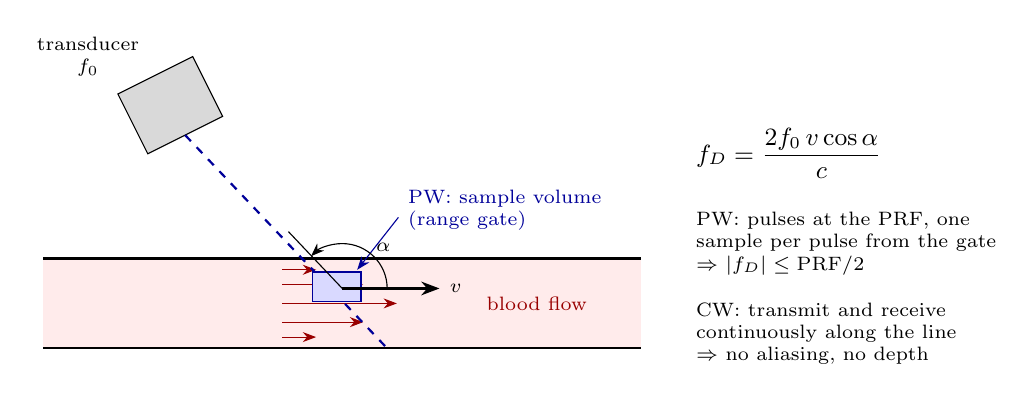
\begin{tikzpicture}[scale=0.95, >=Stealth]
\fill[red!8] (0,0.0) rectangle (8,1.2);
\draw[thick] (0,0) -- (8,0); \draw[thick] (0,1.2) -- (8,1.2);
\foreach \y/\l in {0.15/0.25, 0.35/0.6, 0.6/0.85, 0.85/0.6, 1.05/0.25} {\draw[->, red!60!black] (3.2,\y) -- ++(\l*1.8,0);}
\node[font=\scriptsize, red!60!black] at (6.6,0.6) {blood flow};
\draw[fill=gray!30] (1.0,3.4) -- (2.0,3.9) -- (2.4,3.1) -- (1.4,2.6) -- cycle;
\node[font=\scriptsize, align=center] at (0.6,3.9) {transducer\\$f_0$};
\draw[dashed, thick, blue!60!black] (1.9,2.85) -- (4.6,0.0);
\draw[blue!60!black, fill=blue!15] (3.6,0.62) rectangle (4.25,1.02);
\node[font=\scriptsize, blue!60!black, align=left, anchor=west] at (4.75,1.85) {PW: sample volume\\(range gate)};
\draw[->, blue!60!black, thin] (4.75,1.75) -- (4.2,1.05);
\draw[->, thick] (4.0,0.8) -- (5.3,0.8) node[right, font=\scriptsize] {$v$};
\draw (4.0,0.8) -- ++(-0.72,0.76);
\draw[->] (4.6,0.8) arc (0:134:0.6);
\node[font=\scriptsize] at (4.55,1.35) {$\alpha$};
\node[font=\small, anchor=west] at (8.6,2.6) {$f_D = \dfrac{2 f_0\, v\cos\alpha}{c}$};
\node[font=\scriptsize, anchor=west, align=left] at (8.6,1.4) {PW: pulses at the PRF, one\\sample per pulse from the gate\\$\Rightarrow$ $|f_D| \le \mathrm{PRF}/2$};
\node[font=\scriptsize, anchor=west, align=left] at (8.6,0.2) {CW: transmit and receive\\continuously along the line\\$\Rightarrow$ no aliasing, no depth};
\end{tikzpicture}
\caption{Doppler geometry. The scanner measures the velocity component along the beam.}
\label{fig:geometry}
\end{figure}

\subsection{Pulsed-wave, continuous-wave and tissue Doppler}
\begin{description}[leftmargin=1.2em]
\item[Pulsed wave (PW).] Pulses are sent at the pulse repetition frequency (PRF, a few kHz). After each pulse the
receiver listens for one short time window, which corresponds to one depth: the \emph{sample volume} or range gate.
So PW yields \emph{one complex sample per pulse} from one place. This sequence, indexed by pulse number, is called the
\emph{slow-time signal}. Its sampling rate is the PRF, so by Nyquist the largest unambiguous shift is $\pm$PRF/2,
which by Eq.~\eqref{eq:doppler} is a velocity limit, the \emph{Nyquist velocity}
\begin{equation}
\vnyq = \frac{c\,\mathrm{PRF}}{4 f_0 \cos\alpha}.
\label{eq:nyq}
\end{equation}
Faster flow \emph{aliases}: it appears at the opposite side of the display (Section~\ref{sec:alias}).
\item[Continuous wave (CW).] One half of the transducer transmits continuously and the other half receives. The
signal is not sampled in slow time at the PRF, so there is no practical aliasing and CW can measure the high
velocities of stenotic or regurgitant jets (up to several m/s). The price is that everything along the beam
contributes: CW has no depth resolution.
\item[Tissue Doppler (TDI).] The same PW principle, but tuned to the myocardium: tissue moves slowly (5--20~cm/s)
and reflects strongly, so the filters and gain are set the other way round from blood-flow Doppler. Philips shows
TDI spectra in a copper colour map instead of grey.
\end{description}

\subsection{Why there is a \emph{spectrum} of velocities, and what the envelope is}
The sample volume contains many red cells moving at different speeds. In laminar flow in a tube of radius $R$ the
velocity at distance $r$ from the axis is parabolic, $v(r) = \vmax (1 - r^2/R^2)$, with $\vmax$ the peak velocity on
the axis. If scatterers are spread uniformly over the cross-section, $r^2/R^2$ is uniformly distributed, so the
velocities are \emph{uniformly distributed on $[0,\vmax]$}: every speed from zero up to the peak is present
(Figure~\ref{fig:spectrogram}a). The slow-time signal $z(n)$, with $n$ the pulse number, is the sum of the echoes of
the $N$ scatterers $i = 1\dots N$,
\[
z(n) = \sum_{i=1}^{N} b_i \exp\!\Big(j\big(\phi_i + 2\pi \tfrac{2 f_0}{c} \textstyle\int_0^{n/\mathrm{PRF}} v_i(\tau)\, d\tau\big)\Big) + \text{noise},
\]
where $b_i$ and $\phi_i$ are the random amplitude and phase of scatterer $i$, $v_i(\tau)$ its velocity at time $\tau$,
and $j = \sqrt{-1}$. This is a sum of complex exponentials with random amplitudes and phases
(Figure~\ref{fig:spectrogram}b). Its power spectrum
therefore shows the \emph{distribution of velocities} in the sample volume, weighted by backscattered power.

Because blood accelerates and decelerates during the heartbeat, the distribution changes with time. The scanner
computes a short-time Fourier transform (STFT) of the slow-time signal: windows of $\sim$10--30~ms, a new spectrum
every few ms. Each spectrum becomes one \emph{column} of the display: time runs to the right, velocity runs up and
down, brightness is power. This picture is the \textbf{spectrogram} (Figure~\ref{fig:spectrogram}d).

\begin{figure}[!htbp]
\centering
\includegraphics[width=\linewidth]{spectrogram.pdf}
\caption{From blood flow to a spectrogram (simulation: 300 scatterers in a parabolic profile, PRF 5~kHz,
$f_0$ = 2.5~MHz). (a) A parabolic profile contains every speed from 0 to $\vmax$. (b) The slow-time signal is a
random-looking sum of complex exponentials. (c) Its power spectrum at peak systole is a speckled plateau from 0 to
$\vmax$ that falls into the noise near $\vmax$; the fall is not a sharp step. (d) The spectrogram, with the true
$\vmax(t)$ dashed. The envelope we want is the outer edge of the bright region.}
\label{fig:spectrogram}
\end{figure}

The quantities clinicians measure come from this picture:
\begin{itemize}
\item The \textbf{envelope} or \textbf{maximum velocity} $\vmax(t)$ at time $t$: the outer boundary of the spectrum,
i.e.\ the fastest blood (or tissue) at each moment; $\vmin(t)$ is the same on the negative side. Peak E and A
velocities, jet $V_{\max}$ (the clinical name of the peak of a jet), e$'$ and a$'$, and the
velocity--time integral (VTI) are read from it.
\item The \textbf{mean velocity}: the power-weighted average over the spectrum, i.e.\ the first moment of each column.
\item \textbf{Timing}: onsets, peaks and ends of waves relative to the ECG.
\end{itemize}

\begin{keybox}[Why the envelope is not sharply defined]
Even with perfect hardware, the spectrum does not end in a step. (i) The finite STFT window smears each frequency
over a main lobe (for a 26~ms Hann window, a few cm/s). (ii) Each red cell is inside the beam only briefly, which
broadens its line (\emph{transit-time} or \emph{intrinsic spectral broadening}; worse for fast flow and narrow beams).
(iii) The fastest cells are few, so the outermost part of the spectrum is faint and drowns gradually in noise
(Figure~\ref{fig:spectrogram}c). So ``the'' envelope is a \emph{convention}: where on the fading edge do we draw the
line? Different readers and vendors draw it in different places. This point comes back in
Section~\ref{sec:convention}.
\end{keybox}

\begin{plainbox}
The scanner listens to echoes from moving blood. Moving blood changes the pitch of the echo (the Doppler effect,
like the pitch of a passing ambulance). Because blood in a vessel moves at many speeds at once (fast in the centre,
slow near the wall), the scanner hears a mix of pitches. It shows that mix as a column of grey dots, and draws a new
column every few milliseconds. The bright region is the flow; its outer edge is the fastest blood at that moment.
That edge is what you measure with the caliper, and it is what the program traces.
\end{plainbox}

\section{From spectrum to picture: what the scanner does to the display}
\label{sec:render}

\subsection{Log compression, gain, dynamic range and reject}
Doppler power spans many decades, so the scanner shows it on a logarithmic scale. A simplified grey map is
\begin{equation}
L = 255 \cdot \mathrm{clip}\!\left(\frac{P_{\mathrm{dB}} + G - P_{\mathrm{rej}}}{\mathrm{DR}},\ 0,\ 1\right),
\label{eq:greymap}
\end{equation}
with $L$ the grey level of a pixel (0 = black, 255 = white), $P_{\mathrm{dB}}$ the Doppler power in dB, $G$ the
gain (dB), $P_{\mathrm{rej}}$ the reject level (dB), DR the dynamic range (dB, typically 30--50), and
$\mathrm{clip}(u, a, b) = \min(\max(u, a), b)$, which limits its argument $u$ to $[a, b]$. Three consequences drive the whole method (Figure~\ref{fig:rendering}):
\begin{enumerate}
\item \textbf{Gain is an additive offset} in grey level: $+G$~dB shifts every pixel by $255\,G/\mathrm{DR}$ levels.
Noise and flow shift together. So an absolute grey-level threshold means something different on every image,
whereas \emph{a threshold relative to the noise level} does not (as long as nothing is clipped).
\item \textbf{Reject clips the noise to black.} On most real displays the noise floor is rendered as level 0 with
only the brightest noise specks visible. In 10 of the 17 recent cardiac examples the median level of the display
is exactly 0.
\item \textbf{The original power is unknown.} Gain, reject and dynamic range are not stored in the DICOM. Grey level
is only a monotonic proxy for power. This matters for the mean velocity (Section~\ref{sec:mean}), which needs power.
\end{enumerate}

\begin{figure}[!htbp]
\centering
\includegraphics[width=\linewidth]{rendering.pdf}
\caption{Display rendering of the spectrogram of Figure~\ref{fig:spectrogram} with Eq.~\eqref{eq:greymap}
(DR 40~dB). (a) Gain shifts the grey map sideways. (b, c) The same spectrum at two gains: more gain makes the faint
outer fringe and the noise visible. (d) In the histograms the whole distribution moves up (dotted: medians); at 0~dB
most noise is clipped to black by the reject level.}
\label{fig:rendering}
\end{figure}

\subsection{Everything else on the screen}
The display is a picture made for the human eye, so it carries more than the spectrum (Figure~\ref{fig:screen}):
\begin{itemize}
\item \textbf{The baseline} (zero velocity), drawn as a coloured or grey line, plus time markers and scale ticks.
\item \textbf{Text} (velocity labels, measurements) and sometimes \textbf{the scanner's own envelope trace}.
\item \textbf{The ECG}, drawn as a coloured line along the bottom of the B-mode image. It has no amplitude scale, and
tall R-waves are clipped to its box.
\item \textbf{A sweeping, circular buffer.} The spectrum is written left to right and wraps around. At the write
position there is a gap with no data, the \emph{sweep}. The oldest sample is just right of it.
\item \textbf{Artefacts}: wall-filter clutter (strong, slow signal next to the baseline, partly removed by a
high-pass ``wall'' filter that leaves a dark band), mirror images of strong flow on the opposite side, valve
\emph{clicks} (short, saturated vertical lines when valve leaflets open or close), and aliasing in PW and TDI.
\item \textbf{Different shapes of spectrum}: CW spectra are filled from the baseline up (every velocity along the beam
is present); PW spectra are often \emph{hollow} (the ``spectral window'': in a narrow sample volume of laminar flow,
low velocities are absent); TDI shows thin bands.
\end{itemize}

\begin{figure}[!htbp]
\centering
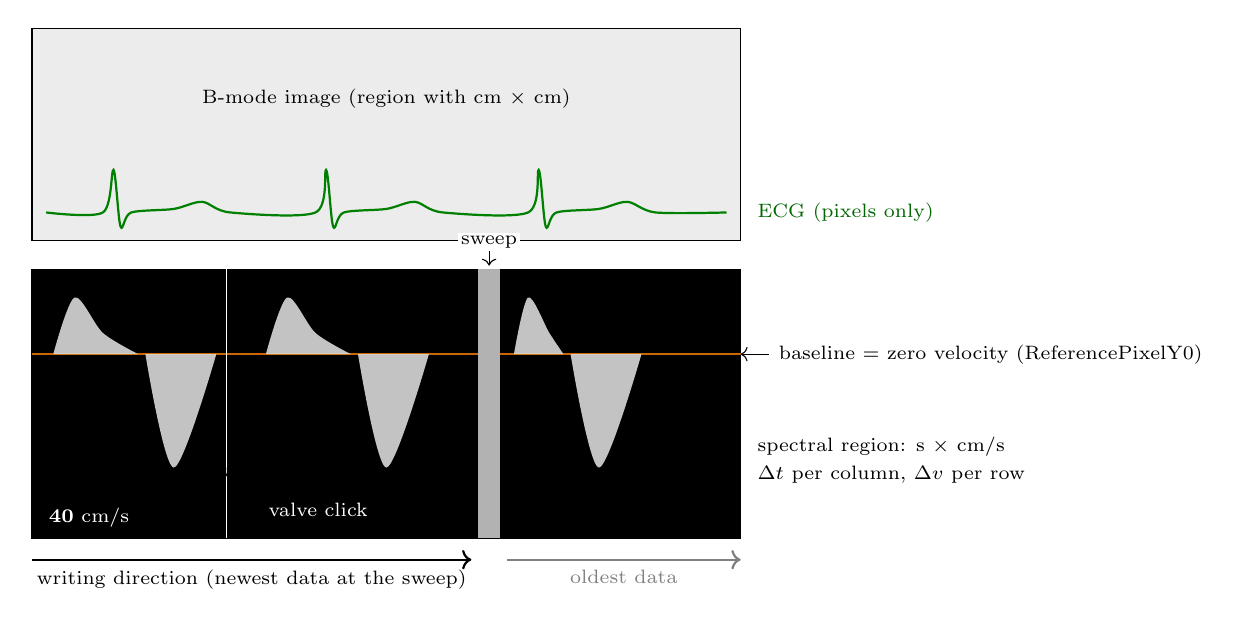
\begin{tikzpicture}[scale=0.9, font=\scriptsize]
\draw[fill=gray!15] (0,4.2) rectangle (10,7.2);
\node at (5,6.2) {B-mode image (region with cm $\times$ cm)};
\draw[green!50!black, thick] plot[smooth] coordinates {(0.2,4.6) (1.0,4.6) (1.15,5.2) (1.25,4.4) (1.4,4.6) (2.0,4.65) (2.4,4.75) (2.8,4.6) (4.0,4.6) (4.15,5.2) (4.25,4.4) (4.4,4.6) (5.0,4.65) (5.4,4.75) (5.8,4.6) (7.0,4.6) (7.15,5.2) (7.25,4.4) (7.4,4.6) (8.0,4.65) (8.4,4.75) (8.8,4.6) (9.8,4.6)};
\node[green!40!black, anchor=west] at (10.1,4.6) {ECG (pixels only)};
\draw[fill=black] (0,0) rectangle (10,3.8);
\draw[orange!80!black, thick] (0,2.6) -- (6.3,2.6); \draw[orange!80!black, thick] (6.6,2.6) -- (10,2.6);
\fill[white!70!gray, opacity=0.9] plot[smooth] coordinates {(0.3,2.6) (0.6,3.4) (1.0,2.9) (1.5,2.6)} -- cycle;
\fill[white!70!gray, opacity=0.9] plot[smooth] coordinates {(3.3,2.6) (3.6,3.4) (4.0,2.9) (4.5,2.6)} -- cycle;
\fill[white!70!gray, opacity=0.9] plot[smooth] coordinates {(1.6,2.6) (2.0,1.0) (2.6,2.6)} -- cycle;
\fill[white!70!gray, opacity=0.9] plot[smooth] coordinates {(4.6,2.6) (5.0,1.0) (5.6,2.6)} -- cycle;
\fill[white!70!gray, opacity=0.9] plot[smooth] coordinates {(7.6,2.6) (8.0,1.0) (8.6,2.6)} -- cycle;
\fill[white!70!gray, opacity=0.9] plot[smooth] coordinates {(6.8,2.6) (7.0,3.4) (7.3,2.9) (7.5,2.6)} -- cycle;
\fill[gray!60] (6.3,0) rectangle (6.6,3.8);
\draw[white] (2.75,0) -- (2.75,3.8);
\node[white, anchor=west] at (0.1,0.3) {\textbf{40} cm/s};
\draw[<-] (6.45,3.85) -- (6.45,4.05) node[above, fill=white, inner sep=1pt] {sweep};
\draw[<-] (10.0,2.6) -- (10.4,2.6) node[right] {baseline = zero velocity (ReferencePixelY0)};
\draw[<-] (2.75,1.0) -- (3.2,0.4) node[right, white] {valve click};
\node[anchor=west] at (10.1,1.3) {spectral region: s $\times$ cm/s};
\node[anchor=west] at (10.1,0.9) {$\Delta t$ per column, $\Delta v$ per row};
\draw[->, thick] (0,-0.3) -- (6.2,-0.3) node[midway, below] {writing direction (newest data at the sweep)};
\draw[->, thick, gray] (6.7,-0.3) -- (10,-0.3) node[midway, below] {oldest data};
\end{tikzpicture}
\caption{Schematic of a spectral Doppler DICOM. Only the pixels are stored; the DICOM header adds the region boxes
and the calibration ($\Delta t$, $\Delta v$, zero row). The circular buffer means the oldest data sit just right of
the sweep.}
\label{fig:screen}
\end{figure}

\subsection{What the DICOM file contains}
The archived DICOM is a single frame: the rendered screen, as an RGB or grey image. There is no raw Doppler signal
and no ECG waveform. What the header does give is the \emph{Ultrasound Region Calibration}: for each region the pixel
box, the physical units of its axes, the time per column $\Delta t$ (2.6--3.5~ms in our files), the velocity per row
$\Delta v$ (from 0.06~cm/s on TDI to 1.7~cm/s on CW), and the row of zero velocity. So the task is an \emph{image}
problem with a ruler attached, not a signal problem.

\begin{plainbox}
The DICOM file we get is essentially a screenshot of the scanner screen, with a hidden ruler that says how many
milliseconds one pixel is to the right and how many cm/s one pixel is up. The original sound signal is gone. The
screenshot also contains things that are not flow: text, the baseline, the ECG line, the moving gap where the screen
is being redrawn, and artefacts. And the brightness depends on the gain the sonographer chose. So the program must
first clean the picture, and must judge brightness \emph{relative to the background noise}, not in absolute terms,
just as an experienced reader does.
\end{plainbox}

\section{Stating the problem precisely}
\label{sec:problem}
The spectral display is $H$ rows high and $W$ columns wide. After calibration we have, for each side of the
baseline, an image $L(k,x)$ of grey levels: column $x = 1\dots W$ is time ($t = x\,\Delta t$), and row
$k = 0\dots D-1$ counts outward from the baseline ($|v| = k\,|\Delta v|$), with $D$ the number of rows on that side.
We want an \emph{edge path} $e = (e_1, \dots, e_W)$, one edge row $e_x$ per column, such that rows $k \le e_x$ hold the
flow's outer part and rows $k > e_x$ hold only noise. With $e^{\mathrm{pos}}_x$ and $e^{\mathrm{neg}}_x$ the edges on
the positive and negative side, $\vmax(x) = e^{\mathrm{pos}}_x |\Delta v|$ and $\vmin(x) = -e^{\mathrm{neg}}_x |\Delta v|$.
The two sides are separate problems.

The obvious solution, ``in each column take the outermost pixel brighter than a threshold'', fails
(Figure~\ref{fig:threshold}). A low threshold catches noise specks far from the flow; a high one cuts the faint
fringe and still jitters from column to column, because each column is decided on its own. Every classical
per-column method (percentile of the integrated spectrum, geometric knee methods, signal--noise slope intersection)
shares this weakness to some degree.

\begin{figure}[!htbp]
\centering
\includegraphics[width=\linewidth]{threshold.pdf}
\caption{Synthetic PW display (SNR 10~dB, speckle, wall clutter; dashed = truth). (a) The outermost pixel above a
threshold, column by column: a low threshold jumps to noise specks, a higher one is ragged and reads low. (b) The
method of this document on the same image (mean error 1.0~cm/s). The short blips near the baseline are wall
clutter just beyond the wall band (Section~\ref{sec:cost}).}
\label{fig:threshold}
\end{figure}

Three ideas fix this, and they are the three stages of the method:
\begin{enumerate}
\item \textbf{Per-pixel evidence relative to the noise} (Section~\ref{sec:memb}): how much does this pixel look like
flow rather than background, independent of gain?
\item \textbf{Neighbourhood evidence} (Section~\ref{sec:dens}): flow comes in patches, noise in isolated specks.
Average the evidence locally.
\item \textbf{A global path with a smoothness prior} (Sections~\ref{sec:cost}--\ref{sec:dp}): choose the edge in all
columns \emph{jointly}, trading off agreement with the evidence against physically implausible jumps. This is solved
exactly by dynamic programming.
\end{enumerate}
Readers with a signal-processing background will recognise the structure: a likelihood term from a detector, and a
Markov prior on the state sequence, solved by the Viterbi algorithm. Section~\ref{sec:bayes} makes this explicit.

%=====================================================================================================
\part{The method, step by step}
\label{part:method}

\begin{figure}[!htbp]
\centering
\begin{tikzpicture}[
  box/.style={draw, rounded corners=2pt, align=center, font=\footnotesize, minimum height=9mm, text width=26mm, fill=#1},
  box/.default=gray!8, arr/.style={-{Stealth[length=2mm]}, thick}, node distance=4mm and 4.5mm]
\node[box=blue!8] (dcm) {DICOM\\pixels + header};
\node[box, right=of dcm] (cal) {\textbf{\S\ref{sec:front}} Region,\\calibration};
\node[box, right=of cal] (clean) {\textbf{\S\ref{sec:front}} Cleaning: overlays,\\text, sweep, clicks};
\node[box=orange!12, right=of clean] (memb) {\textbf{\S\ref{sec:memb}} Noise stats,\\soft membership $m$};
\node[box=orange!12, below=of memb] (dens) {\textbf{\S\ref{sec:dens}} Local density $d$\\(bg-subtracted, normalised)};
\node[box=orange!12, left=of dens] (cost) {\textbf{\S\ref{sec:cost}} Edge cost\\$C_x(k)$ per column};
\node[box=orange!12, left=of cost] (dp) {\textbf{\S\ref{sec:dp}} DP: best smooth\\path per side};
\node[box, left=of dp] (alias) {\textbf{\S\ref{sec:alias}} Aliasing?\\unwrap, redo};
\node[box, below=of alias] (mean) {\textbf{\S\ref{sec:mean}} Mean velocity\\in flow region};
\node[box=green!6, right=of mean] (ecg) {\textbf{\S\ref{sec:ecg}} ECG, R-peaks,\\clicks, AVC};
\node[box=green!12, right=of ecg, text width=40mm] (out) {$t$, ECG, $\vmax$, $\vmin$, $v_{mean}$,\\R-peaks, AVC, flags};
\draw[arr] (dcm) -- (cal); \draw[arr] (cal) -- (clean); \draw[arr] (clean) -- (memb);
\draw[arr] (memb) -- (dens); \draw[arr] (dens) -- (cost); \draw[arr] (cost) -- (dp); \draw[arr] (dp) -- (alias);
\draw[arr] (alias) -- (mean); \draw[arr] (mean) -- (ecg); \draw[arr] (ecg) -- (out);
\end{tikzpicture}
\caption{The pipeline (\code{extract\_waveforms()}). Orange: the envelope estimator, the core of this document.
About 0.2~s per 1024$\times$768 image.}
\label{fig:pipeline}
\end{figure}

\section{Front end: calibration and cleaning}
\label{sec:front}
These steps are bookkeeping, but each one prevents a specific failure.
\begin{itemize}
\item \textbf{Find the spectral region by its units} (\code{spectral\_region}): the region whose x axis is seconds
and y axis is cm/s. The order of regions in the header differs between files, so it is never used.
\item \textbf{Zero-velocity row} = header \code{ReferencePixelY0}. The header wins over detecting the drawn line,
which can lock onto saturated flow. The sign of $\Delta v$ (\code{PhysicalDeltaY}) is kept, so if the operator
inverted the display the output sign follows the header, not the on-screen label.
\item \textbf{Overlays are masked, then filled} (\code{build\_spectrogram}): coloured pixels on a grey display (ECG,
markers, vendor trace), grey pixels on a colour-map display, the baseline colour, and white text, recognised as
\emph{small bright blobs with a dark surround} (saturated flow and clicks have a bright surround). Masked pixels are
filled by linear interpolation along the column, so they neither add nor remove evidence. Setting them to zero
would punch dark holes into the flow.
\item \textbf{Colour map}: TDI copper colours are converted to a level by luminance $\times 255/160$ (the brightest
copper colour has luminance $\approx$150), so grey and colour displays share one scale.
\item \textbf{Sweep and time order}: columns where the drawn baseline is missing (runs $\ge$3~px) are the sweep. They
are marked invalid (never interpolated, output NaN). All outputs are rotated so time runs oldest $\to$ newest.
\item \textbf{Modality}: CW from the header's region data type, TDI from a colour map or a display range below
40~cm/s, PW otherwise.
\item \textbf{Valve clicks} are detected here (Section~\ref{sec:ecg}). By default (\code{click\_mode: keep}) the
display is left as it is, so the envelope traces the clicks as shown.
\end{itemize}

\begin{plainbox}
Before looking for the flow, the program uses the hidden ruler to find the Doppler strip and the zero line, rubs out
everything drawn on top (text, ECG, markers) by filling it in from the pixels above and below, ignores the moving gap
where the screen is redrawn, and puts the pieces of the recording in the right time order.
\end{plainbox}

\section{Step 1 --- How flow-like is each pixel? (soft membership)}
\label{sec:memb}

\subsection{Robust noise statistics}
Flow occupies a minority of the display area, so most pixels are background. Statistics that ignore the minority are
therefore noise statistics. The code (\code{noise\_stats}) uses, over the grey levels $L$ of all valid pixels
(not overlay, not sweep):
\begin{align}
\mu &= \mathrm{median}(L), \qquad \sigma = 1.4826\,\mathrm{median}\big(|L-\mu|\big),
\end{align}
the median $\mu$ (the noise level) and the scaled median absolute deviation (MAD) $\sigma$ (the noise spread). The
factor 1.4826 makes $\sigma$ equal the standard deviation for Gaussian data; unlike the mean and standard deviation,
neither statistic is pulled by the bright flow pixels. It also computes Otsu's threshold $T_{\mathrm{Otsu}}$: the grey
level that splits the histogram into a dark and a bright class with maximal between-class variance
$\omega_0 \omega_1 (\bar L_1 - \bar L_0)^2$, where $\omega_0, \omega_1$ are the fractions of pixels in the two classes
and $\bar L_0, \bar L_1$ their mean grey levels.

\subsection{The threshold and the ramp}
From these the code sets a \emph{signal threshold} $T$ (membership reaches 1) and a \emph{noise top} $T_0$
(membership starts to rise):
\begin{equation}
T = \min\!\big(\mu + \max(M,\ \beta\sigma),\ T_{\mathrm{Otsu}}\big), \qquad T_0 = \mu + \gamma\,\max(\sigma, 1),
\end{equation}
with the noise margin $M = 32$ grey levels, the noise-spread factor $\beta = 4$ and the soft-start factor
$\gamma = 1.5$. Each pixel $(k,x)$ gets a \emph{soft membership}
\begin{equation}
m(k,x) = \mathrm{clip}\!\left(\frac{L(k,x) - T_0}{\max(T - T_0,\, 1)},\ 0,\ 1\right),
\label{eq:memb}
\end{equation}
which is 0 for noise, 1 for clear signal and ramps linearly in between (Figure~\ref{fig:membership}).

\begin{itemize}
\item \emph{Why relative to $\mu$}: by Eq.~\eqref{eq:greymap}, gain shifts $L$ and $\mu$ equally, so $L-\mu$ and hence
$m$ do not change. The threshold is gain-invariant as long as the noise is not clipped (see the note below).
\item \emph{Why $\max(M, \beta\sigma)$}: the threshold must clear the noise by a fixed margin \emph{and} by
several noise standard deviations, whichever is larger.
\item \emph{Why the Otsu cap}: on very dense displays (a CW jet filling much of the strip) the median is no longer
pure noise and $\mu + \beta\sigma$ can land inside the flow. Otsu, which separates the two populations, then keeps $T$
sensible.
\item \emph{Why soft}: a hard threshold makes faint flow all-or-nothing. With the ramp a faint pixel counts
partially, so the faint fringe still pulls the edge outward a little. This was the main improvement over the first
(MATLAB) version of the tracer.
\end{itemize}

\begin{figure}[!htbp]
\centering
\includegraphics[width=\linewidth]{membership.pdf}
\caption{(a) Level histogram of the synthetic display (log scale) and the membership ramp (red, right axis). As on
most real displays the noise is rendered black, so $\mu = \sigma = 0$, $T_0 = 1.5$, and $T = \min(M, T_{\mathrm{Otsu}}) = 20$.
(b) The membership image: the flow is bright, but so are many isolated noise specks.}
\label{fig:membership}
\end{figure}

\begin{notebox}[Two subtleties found while writing this document]
\textbf{Black noise.} When reject renders the noise black (10 of 17 real cardiac examples), $\mu = \sigma = 0$ and
$T = \min(M, T_{\mathrm{Otsu}})$ is effectively an absolute threshold. Gain invariance then holds only partly:
more gain lifts the faint fringe above $T$ and moves the edge outward, much as it does for a human reader.

\textbf{Collapsed ramp.} If the Otsu cap pulls $T$ below $T_0$ (possible when $\sigma$ is large), the denominator
in Eq.~\eqref{eq:memb} becomes 1 and the ramp turns into a hard step at $T_0$, above the intended threshold. This
happened in 3 of the 17 real examples (one PW, two CW with bright noise). The density stage absorbs much of the
effect. The obvious fix, $T_0 \leftarrow \min(T_0, T-1)$, made one of the three worse, so the default is unchanged.
\end{notebox}

\begin{plainbox}
The program first asks of every dot: is this brighter than the background speckle? It learns what ``background''
looks like from the picture itself (most of the strip is background). A dot well above the background counts as
flow, a dot at background level counts as nothing, and a dot in between counts partly. Because everything is
judged relative to the background, turning the gain up or down changes little.
\end{plainbox}

\section{Step 2 --- From pixels to patches (local density)}
\label{sec:dens}

\subsection{Local averaging}
Membership alone is noisy: isolated specks score 1, and dark gaps inside speckled flow score 0. Real flow differs
from noise in being \emph{spatially coherent}. The code (\code{DPEstimator.likelihood}) therefore averages $m$ over a
small box,
\begin{equation}
\tilde d(k,x) = \frac{1}{9\cdot 5}\sum_{|\delta k|\le 4}\ \sum_{|\delta x| \le 2} m(k+\delta k,\, x+\delta x),
\end{equation}
the \emph{local mean} $\tilde d$, with $\delta k$ and $\delta x$ the row and column offsets within the box:
9 rows by 5 columns ($\approx$5~cm/s $\times$ 18~ms on a $\pm$100~cm/s PW display). In signal-processing terms this is
a 2-D moving-average (low-pass) filter. Its value is the \emph{fraction of flow-like pixels} in the neighbourhood: an
isolated speck gives $1/45$, the inside of a flow region gives close to 1.

\subsection{Background subtraction and normalisation}
Two corrections turn $\tilde d$ into the \emph{density} $d$ used by the cost. With $Q_q(\cdot)$ the $q$-th percentile
over all valid pixels,
\begin{align}
d' &= \mathrm{clip}\!\left(\frac{\tilde d - d_{\mathrm{bg}}}{1-d_{\mathrm{bg}}},\, 0,\, 1\right), \quad d_{\mathrm{bg}} = Q_{50}(\tilde d)\quad(\text{applied if } d_{\mathrm{bg}}<0.9),\\
d  &= \mathrm{clip}\!\left(\frac{d'}{\max(Q_{99}(d'),\ 0.1)},\, 0,\, 1\right),
\end{align}
where $d_{\mathrm{bg}}$ is the background density, $d'$ the background-subtracted density, and 0.1 a floor that stops
a nearly empty image from being blown up.
\begin{itemize}
\item \textbf{Background subtraction.} The median density is the typical density of the background. Subtracting it
makes background pixels exactly 0. Without it, uniform noise has a small positive density everywhere, and as the next
section shows, every positive density beyond the edge is a reason to move the edge outward: at low SNR the edge then
runs to the display limit.
\item \textbf{Normalisation.} The 99th percentile is the density in the core of the flow. Dividing by it maps ``typical
in-flow density'' to 1 on every image. A dense CW jet and a speckled TDI band both end up with cores near 1, so a
single \emph{edge level} $\theta$ (default 0.5, used in the next section) means the same thing on both: \emph{the
edge lies where the density has fallen to the fraction $\theta$ of the core density}. Without normalisation, $\theta = 0.5$ cut faint TDI and $\theta = 0.2$ read
3--11~cm/s too far out on vascular PW.
\item \textbf{TDI only}: each side is also divided by its running column maximum over $\pm$10~ms (floor 0.15), so
faint, slow tissue segments are not lost next to bright ones.
\end{itemize}

\begin{figure}[!htbp]
\centering
\includegraphics[width=\linewidth]{density.pdf}
\caption{One beat of the synthetic display. (a) Membership. (b) After the 9$\times$5 moving average, isolated specks
fade and the flow becomes a coherent region. (c) After background subtraction and normalisation; green: the contour
$d = \theta = 0.5$, which is roughly where the edge will be placed.}
\label{fig:density}
\end{figure}

\begin{plainbox}
One bright dot on its own is probably noise; a patch of bright dots is probably flow. So the program replaces each
dot by ``how many of its neighbours look like flow''. Then it rescales the picture so that the inside of the flow
counts as 100\,\%, whatever the scanner, gain or type of recording. From here on it works with this cleaned-up map of
``flow-likeness'' instead of the raw picture.
\end{plainbox}

\section{Step 3 --- Where does the flow end in one column? (the edge cost)}
\label{sec:cost}

\subsection{The cost of a candidate edge}
Take one column of the density, $d_{k'} = d(k', x)$ for rows $k' = 0\dots D-1$ outward from the baseline, and a
candidate edge row $k$. The code (\code{edge\_cost}) scores the candidate by
\begin{equation}
C(k) = \underbrace{\sum_{k'>k} \big(d_{k'} - \theta\big)_+}_{\text{(i) signal left outside}}
\;+\; \underbrace{\sum_{k-h<k'\le k} w_{k'}\,\big(\theta - d_{k'}\big)_+}_{\text{(ii) no signal just inside}}
\;+\; \underbrace{\rho\,k}_{\text{(iii) weak prior}},
\label{eq:cost}
\end{equation}
with $(u)_+ = \max(u, 0)$; the edge level $\theta = 0.5$; the inner band $h$ = 5\,\% of the display height $H$
($\approx$19 rows); the height prior $\rho = 0.01$; and the wall weight $w_{k'} = 0.01$ inside the wall band (3\,\% of
$H$ next to the baseline), $w_{k'} = 1$ elsewhere. When the column matters we write $C_x(k)$ for the cost of edge
row $k$ in column $x$.
Read it as the number of ``errors'' the candidate would make (Figure~\ref{fig:cost}):
\begin{enumerate}[label=(\roman*)]
\item Every pixel \emph{beyond} the edge that is denser than $\theta$ is flow left outside. Moving the edge outward past
it removes this cost. Pixels with $d < \theta$ beyond the edge cost nothing, so moving the edge outward
\emph{through noise never lowers the cost}.
\item Every pixel in a band of $h$ rows \emph{just inside} the edge that is less dense than $\theta$ is ``no flow inside
the flow''. This stops the edge from drifting outward into empty space: an edge must sit on top of signal.
\item A tiny cost per row of edge height. On a column with no flow at all (all $d < \theta$) terms (i) and (ii) are
flat, and this term makes the answer $k = 0$: no flow.
\end{enumerate}
Each wrongly classified pixel costs at most 0.5 (since $\theta = 0.5$), and the prior adds 1.15 for an edge at
60~cm/s on a $\pm$100~cm/s display, so the prior only breaks ties.

\subsection{Why only a band just inside the edge}
The interior deeper than $h$ rows is \emph{free}: the cost does not care whether it is filled. This is the key
difference from the earlier MATLAB tracer, which used a \emph{two-region split},
$C_{\mathrm{split}}(k) = \sum_{k'>k} d_{k'} + \sum_{k'\le k} (1-d_{k'})$: ``everything outside should be empty and everything
inside should be full''. That is right for CW (filled spectra), but a hollow PW spectrum or a thin TDI band has a large
empty interior, and the split then prefers to put the edge at the baseline (Figure~\ref{fig:cost}c,d: 2~cm/s instead
of 60). The outer-edge cost asks only what defines an outer edge: dense on the inside of the boundary, empty beyond
it.

\begin{figure}[!htbp]
\centering
\includegraphics[width=\linewidth]{column_cost.pdf}
\caption{The edge cost on two constructed density columns with the same outer edge (60~cm/s) and a noise blob near
85~cm/s. Left: density and the chosen edges (blue = edge cost, dashed = old two-region split). Right: the three
terms of Eq.~\eqref{eq:cost} and their sum. The noise blob adds term (i) above 60~cm/s, but jumping out to it would
cost more in term (ii) (the empty band between). On the hollow column the old split collapses to the baseline.}
\label{fig:cost}
\end{figure}

\subsection{The wall band}
Near the baseline the wall filter leaves either a dark gap or bright clutter. In the lowest 3\,\% of rows term (ii)
is weighted by 0.01, so a dark gap there does not count against an edge. After the path is found, an edge that ends
\emph{inside} the wall band is reported as 0: there is no detectable flow, only clutter. Clutter that extends slightly
beyond the band appears as short low blips (visible in Figure~\ref{fig:threshold}b).

\subsection{Efficient evaluation}
For all $k$ at once, (i) is a reversed cumulative sum and (ii) a difference of cumulative sums $h$ rows apart, so
$C$ for a whole image costs $O(DW)$.

\begin{plainbox}
For one moment in time (one column), the program considers every possible height for the edge and counts the
mistakes each would make: flow left outside the line, or empty space just inside it. The best height is where flow
stops and nothing comes after it. The inside of the spectrum does not need to be filled, so hollow PW spectra and the
thin bands of tissue Doppler work too. If a column holds no flow at all, the answer is zero.
\end{plainbox}

\section{Step 4 --- Linking the columns: the smoothness prior and dynamic programming}
\label{sec:dp}

\subsection{The energy}
Choosing the minimum of $C_x(k)$ in each column separately still gives a jittery edge that jumps to strong noise
blobs (Figure~\ref{fig:dptoy}a, orange crosses; Figure~\ref{fig:clin}, panel 3). Blood has inertia: its velocity
cannot change arbitrarily fast. So the edge path $e = (e_1, \dots, e_W)$ of each side is chosen to minimise the
\emph{energy}
\begin{equation}
E(e) = \sum_{x=1}^{W} C_x(e_x) \;+\; \lambda \sum_{x=2}^{W} |e_x - e_{x-1}|.
\label{eq:energy}
\end{equation}
The first term rewards agreement with the evidence; the second penalises moving the edge between neighbouring columns,
with the \emph{smoothness weight} $\lambda$ as the price per row moved.

\subsection{The smoothness weight as a physical acceleration}
Moving the edge by one row between neighbouring columns means a velocity change of $|\Delta v|$ in $\Delta t$, an
acceleration of $|\Delta v|/\Delta t$. The code sets
\begin{equation}
\lambda = \frac{|\Delta v| / \Delta t}{a_{\mathrm{ref}}}, \qquad a_{\mathrm{ref}} = a_0\,\frac{V_{\mathrm{disp}}}{100~\mathrm{cm/s}},
\quad a_0 = 640~\mathrm{cm/s^2},
\label{eq:lambda}
\end{equation}
with $a_{\mathrm{ref}}$ the \emph{reference acceleration}, $a_0$ its value for a display range of 100~cm/s, and
$V_{\mathrm{disp}}$ the largest $|v|$ on the display. If the edge moves by $\Delta e = e_x - e_{x-1}$ rows, its
acceleration is $a = |\Delta e|\,|\Delta v|/\Delta t$ and the smoothness cost of that step is
$\lambda\,|\Delta e| = a/a_{\mathrm{ref}}$: an edge accelerating at exactly $a_{\mathrm{ref}}$ pays 1 per column, the
price of two fully misclassified pixels. Faster changes are allowed when the evidence pays for them.

\begin{keybox}[What $\lambda$ is in practice]
On a symmetric display $|\Delta v| \approx 2V_{\mathrm{disp}}/H$, so Eq.~\eqref{eq:lambda} gives
$\lambda \approx 200/(H\,\Delta t\,a_0)$: the display range cancels. For $H = 385$ rows and $\Delta t = 3.5$~ms,
$\lambda \approx 0.23$ on PW ($\pm$100~cm/s), CW and TDI ($\pm$15~cm/s) alike. Scaling with the range was introduced
because a fixed $a_{\mathrm{ref}}$ clipped the steep upstrokes of high-velocity jets; its effect is that the prior is
really defined \emph{in fractions of the display range per second}: the edge may cross the full range $V_{\mathrm{disp}}$
in about $100/640 \approx 0.16$~s at the cost-neutral rate. Since sonographers set the scale to fit the flow, this is
a sensible, scale-free prior.
\end{keybox}

\emph{Why L1 and not squared differences.} The $|\Delta e|$ penalty is a total-variation prior. It charges a jump of
$|\Delta e|$ rows the same whether it happens at once or in steps, so it does not round off abrupt events such as valve
opening; a quadratic penalty would charge $\Delta e^2$ and smear such onsets. The effect of $a_{\mathrm{ref}}$ is shown in
Figure~\ref{fig:lambda}.

\begin{figure}[!htbp]
\centering
\includegraphics[width=\linewidth]{lambda.pdf}
\caption{Effect of $a_{\mathrm{ref}}$ on one beat of the synthetic display. Without smoothness ($\lambda \approx 0$)
each column decides alone and picks up spurious blips. With the default the edge follows the truth (dashed). A very
low $a_{\mathrm{ref}}$ (stiff path) cannot follow the steep upstroke and clips the peak.}
\label{fig:lambda}
\end{figure}

\subsection{Solving it exactly: dynamic programming}
Equation~\eqref{eq:energy} has $D^W$ candidate paths (about $385^{900}$), but it has \emph{chain structure}: each term
involves at most two neighbouring columns. Define the \emph{value function} $F_x(k)$ as the lowest energy of any path
over columns $1\dots x$ that ends at row $k$. Then
\begin{equation}
F_1(k) = C_1(k), \qquad F_x(k) = C_x(k) + \min_{k'} \big[F_{x-1}(k') + \lambda |k-k'|\big],
\label{eq:dp}
\end{equation}
and we store the minimising $k'$ (the best row in the previous column) as a \emph{back-pointer} $B_x(k)$. After the
last column, $e_W = \arg\min_k F_W(k)$, and backtracking $e_{x-1} = B_x(e_x)$ recovers the whole path (\code{dp\_solve}). Because every path's energy decomposes this
way, the result is the \textbf{global minimum} of Eq.~\eqref{eq:energy}, not a local one, and it needs no
initialisation. Figure~\ref{fig:dptoy}a shows a toy example: the per-column minima jump to a bright speck at row 7 and
a dropout to row 0; the DP path pays a little in those columns and saves much more in transition cost.

\begin{figure}[!htbp]
\centering
\includegraphics[width=\linewidth]{dp_toy.pdf}
\caption{(a) Toy cost table: per-column minima (orange) versus the DP path (red), which minimises cost plus
$\lambda\times$jumps. (b) The inner minimum of Eq.~\eqref{eq:dp} is the lower envelope of cones of slope $\lambda$
centred on the previous column's $F$ values; it is computed in two linear passes.}
\label{fig:dptoy}
\end{figure}

\subsection{Making it fast: the L1 distance transform}
Evaluated naively, the inner minimum of Eq.~\eqref{eq:dp} costs $O(D^2)$ per column. For an L1 penalty it is a
\emph{distance transform} (Felzenszwalb and Huttenlocher). Write $g(k') = F_{x-1}(k')$ and
$\psi(k) = \min_{k'} g(k') + \lambda|k-k'|$ for the inner minimum. Then
\begin{align*}
\text{forward:}\quad & \psi(0) = g(0),\quad \psi(k) = \min\big(g(k),\ \psi(k-1) + \lambda\big),\\
\text{backward:}\quad & \psi(k) \leftarrow \min\big(\psi(k),\ \psi(k+1) + \lambda\big)
\end{align*}
gives $\psi$ exactly: any optimal $k'$ is reached by walking from $k'$ to $k$ one row at a time, paying $\lambda$ per
row, in one of the two directions. Geometrically, $\psi$ is the lower envelope of cones (Figure~\ref{fig:dptoy}b). The
code computes the same two passes with cumulative minima of $g(k') \mp \lambda k'$
(\code{\_l1\_min\_convolution}), tracking the argmin for the back-pointers. The whole DP is $O(DW)$: a few ms per side.

\subsection{Details: sweep, confidence, output}
\begin{itemize}
\item \textbf{Sweep.} Columns on either side of the sweep are not adjacent in time, so the transition into a sweep
column (and out of it) is free, and sweep columns have zero cost. The path there is meaningless and the output is NaN.
\item \textbf{Confidence.} For each column the code reports
$\big(\overline{C_x} - C_x(e_x)\big)/\big(\max_k C_x(k) - \min_k C_x(k)\big) \in [0,1]$, with $\overline{C_x}$ the mean
of $C_x(k)$ over all rows $k$ (\code{conf\_pos}, \code{conf\_neg}): how much better the chosen edge is than an average
candidate.
\item \textbf{Output.} $\vmax = e^{\mathrm{pos}}|\Delta v|$, $\vmin = -e^{\mathrm{neg}}|\Delta v|$.
\end{itemize}

\subsection{The same thing, seen as Bayesian estimation}
\label{sec:bayes}
Write $\Pr(e \mid \text{image}) \propto \prod_x \exp(-C_x(e_x)) \prod_x \exp(-\lambda|e_x - e_{x-1}|)$. The first factor is a
per-column likelihood, the second a random-walk prior with Laplace-distributed increments (scale $1/\lambda$ rows).
Minimising $E$ is maximising this posterior (MAP). Equivalently, it is a hidden Markov model whose hidden state is the
edge row, with transition probabilities $\propto \exp(-\lambda|\Delta e|)$ and emission log-likelihood $-C_x(k)$; the
DP of Eq.~\eqref{eq:dp} is the Viterbi algorithm. This is the same machinery as pitch or ridge tracking in speech
spectrograms. What is specific to Doppler here is the data term (outer edge, free interior, normalised
noise-referenced density) and the prior in physical units.

\begin{plainbox}
Deciding each moment on its own gives a jagged line that jumps to stray specks. So the program does what a careful
reader does by eye: it looks at the whole recording at once and draws one smooth line. Technically, it considers
\emph{every} possible line through the picture and picks the one with the fewest mistakes, where a mistake is
either disagreeing with the picture or changing speed faster than blood plausibly can. That sounds impossible
(there are astronomically many lines), but a classic trick, dynamic programming, finds the best line exactly in a
fraction of a second. Think of a satellite navigation system that plans the best route over the whole map instead of
choosing each turn on the spot. A sudden real change, such as a valve opening, is still allowed when the picture
clearly shows it.
\end{plainbox}

\section{Aliasing: detection and automatic unwrapping}
\label{sec:alias}

\subsection{Why PW spectra wrap around}
PW samples the slow-time signal at the PRF. Sampling makes the spectrum periodic with period PRF, i.e.\ periodic in
velocity with period $2\vnyq$ (Eq.~\eqref{eq:nyq}). The display shows one period. A baseline shift moves the window
but does not change its span. Flow faster than one limit therefore re-enters from the other limit
(Figure~\ref{fig:alias}a). Clinically this is the ``wrap-around'' that sonographers fix by shifting the baseline or
raising the scale. CW is not sampled this way and is never tested.

\subsection{Detection: the wrap-around test}
Wrapped flow leaves the display at one limit and re-enters at the other \emph{in the same columns}, so after the first
DP pass both edges sit at their display limits. The test (\code{aliasing\_suspected}) fires if, in more than 1\,\% of the
data columns, both edges are within 2\,\% of their limits. One edge alone at its limit is common (clutter or a mirror
filling a small side) and is not counted.

\subsection{Correction: a least-signal cut on the circular display}
The fix mimics a baseline shift that may vary from column to column (\code{find\_cut}, \code{unwrap}):
\begin{enumerate}
\item Treat each column as circular: the row below the bottom limit is the top limit. Exclude a guard band of 10\,\%
of the height on each side of the baseline.
\item Find, by the same DP solver, a \emph{cut path} through this circular coordinate that crosses as little
(smoothed) density $d$ as possible. Cost per pixel: the density, plus 0.002 per row of distance from the display edge
(so with no evidence the cut stays at the edge, i.e.\ no change). Cost per move between columns: $\lambda_{\mathrm{cut}}
= 0.05$ per row moved, plus $\kappa = 0.25$ per unit of density the cut passes over on the way, counting only density
present in \emph{both} columns. The second term stops the cut from jumping through a flow band to the band's other
side, while following a band that grows is free. Without it the cut sometimes took a shortcut through the empty
spectral window of a hollow PW spectrum and unwrapped a beat the wrong way (one beat in 3 of 8 synthetic test
seeds). It keeps the DP linear: the move cost is still a distance $|\xi(k) - \xi(k')|$ between rows, measured in a
warped row coordinate $\xi(k) = \lambda_{\mathrm{cut}} k + \kappa \sum_{k'' \le k} \min\big(d_{x-1}(k''), d_x(k'')\big)$,
so the distance transform of Section~\ref{sec:dp} applies with $\xi$ in place of $\lambda k$.
\item Accept only if the cut crosses less than half the density found at the display edge (and that edge density is
above 0.05): there must be real flow at the edge and a real gap at the cut.
\item Move the rows beyond the cut by one display span. The image becomes taller; the wrapped flow joins the flow it
belongs to. Then Steps 1--4 run again on the unwrapped image, so $\vmax$ or $\vmin$ may exceed the display limits.
\end{enumerate}

\begin{figure}[!htbp]
\centering
\includegraphics[width=\linewidth]{aliasing.pdf}
\caption{(a) Sampling at the PRF creates spectral replicas every $2\vnyq$; the display shows one period, so the part
of the true spectrum beyond $+\vnyq$ appears near $-\vnyq$. (b) Synthetic PW display with a $-40$~cm/s limit and a
$-75$~cm/s systolic jet: the first pass hits both limits. Green dots: the least-signal cut (at $+100$ and $-40$~cm/s
it is at the display edge, which is the same point on the circle, meaning ``no change''). (c) After moving the rows
beyond the cut, the jet is traced to its true depth (dashed white); dotted: original display limits.}
\label{fig:alias}
\end{figure}

\begin{notebox}[Limits]
Flow whose total spread in one column exceeds the display span cannot be unwrapped. With the density-crossing term
($\kappa$) all beats of the 8 synthetic test seeds are unwrapped (before: one beat in 3 seeds stayed wrapped); on the
real examples it changed one column of one image by 2.8~cm/s. The flags \code{aliasing\_suspected} and
\code{aliasing\_corrected} let you spot doubtful cases.
\end{notebox}

\begin{plainbox}
When the flow is faster than the scale allows, PW Doppler ``wraps around'': the top of the wave reappears at the
bottom of the screen (like wagon wheels that seem to turn backwards in a film). The program notices this because the
traced line hits the top and bottom of the screen at the same moment. It then does what the sonographer would do with
the baseline shift, but separately for every moment: it finds the quietest place to ``cut'' the picture, moves the
wrapped part back where it belongs, and traces again.
\end{plainbox}

\section{Mean velocity}
\label{sec:mean}
The scanner's mean velocity is the first moment of the power spectrum. From the display we can only approximate it
(\code{mean\_envelopes}):
\begin{enumerate}
\item \textbf{De-compress} the grey level to relative power by inverting Eq.~\eqref{eq:greymap} with an assumed
dynamic range $\mathrm{DR} = 40$~dB: $P(L) = 10^{L\,\mathrm{DR}/2550} - 1$ is the relative power of a pixel with grey
level $L$. Each pixel gets the weight $p = \max\big(P(L) - P(\mu), 0\big)$, its power above the noise power $P(\mu)$.
\item \textbf{Restrict to the flow region}: rows between the baseline (excluding the zero row) and the traced edge.
Noise outside the flow, if included, would pull the mean toward the middle of the display.
\item Per column, $v_{\mathrm{mean,pos}} = \sum p\,v / \sum p$ over the pixels of the positive flow region, with $v$ the
velocity of each pixel's row; $v_{\mathrm{mean,neg}}$ likewise on the negative side; $v_{\mathrm{mean}}$ over both (signed).
A side without flow gets 0.
\end{enumerate}
The assumed DR is not in the DICOM, so this is a proxy; it is validated only on synthetic data ($\sim$1\,\% of the
display span), see Figure~\ref{fig:mean}.

\begin{figure}[!htbp]
\centering
\includegraphics[width=\linewidth]{mean.pdf}
\caption{(a) One column: de-compressed power over velocity; only the part inside the traced edge (blue) is
averaged. (b) Over time, the estimated mean follows the true power-weighted mean on synthetic data.}
\label{fig:mean}
\end{figure}

\begin{plainbox}
Besides the fastest blood (the edge), the program also estimates the average speed of all the blood at each moment,
giving brighter parts of the spectrum more weight. Because the scanner's brightness settings are not stored, this
average is an approximation, unlike the edge.
\end{plainbox}

\section{Timing: ECG, R-peaks, valve clicks and aortic valve closure}
\label{sec:ecg}
The downstream analyses use the timing between ECG and Doppler events, so these share the envelope's time axis.
\begin{itemize}
\item \textbf{ECG trace} (\code{extract\_ecg}). In a band of rows along the lower edge of the B-mode region, the
trace is the colour that spans most columns without being a horizontal line (the baseline colour is excluded).
Per column the code samples the stroke top or bottom at local extremes (so R and S keep their amplitude) and the
stroke centre elsewhere; gaps up to 50~ms are interpolated, never across the sweep. Amplitude is in pixels,
normalised to $\max|\mathrm{ECG}| = 1$; only timing is meaningful. Flat runs at the extreme row raise
\code{ecg\_clipped}.
\item \textbf{R-peaks} (\code{detect\_rpeaks}), Pan--Tompkins style: zero-phase 8--30~Hz band-pass (the QRS band),
squared in robust-SD units and smoothed over 100~ms. Using QRS-band \emph{energy} rather than amplitude stops tall
T-waves from being counted. Peaks need a 250~ms refractory period and at least 0.35$\times$ the median of the upper
half of the candidate peak heights (strips hold only 2--8 beats). In RR gaps longer than 1.66$\times$ the expected RR
(from the DICOM \code{HeartRate} tag if present) a search-back adds the most plausible missed beat; a T-wave guard
removes small peaks at 20--55\,\% of RR. Each peak is refined to the largest deflection within $\pm$40~ms.
\item \textbf{Valve clicks} (\code{find\_clicks}): short broadband transients, i.e.\ bright vertical lines. Take the
column-mean level and apply a white top-hat (signal minus its morphological opening) with a flat 35~ms structuring
element: this removes slow variations and steps (flow onset) and keeps only features narrower than 35~ms. Columns
above 12 robust SDs in runs no wider than 35~ms are clicks.
\item \textbf{Aortic valve closure (AVC)} (\code{aortic\_valve\_closure}): per beat, the strongest click transient
0.20--0.50~s after the R-peak, at least 6 robust SDs, not at the window edges, timed at the half-maximum centroid.
\end{itemize}

\begin{figure}[!htbp]
\centering
\includegraphics[width=\linewidth]{overview.pdf}
\caption{All outputs of one synthetic CW recording on a shared time axis. With the default \code{click\_mode: keep}
the envelopes follow the clicks as drawn (the vertical spikes); the click times are reported separately, and the
R-gated strongest click per beat is the AVC.}
\label{fig:overview}
\end{figure}

\begin{plainbox}
The ECG on the screen is just a drawn line, so the program traces it by its colour and finds the R-waves by looking
for the sharp burst of energy of each QRS complex (so a tall T-wave is not mistaken for an R-wave). Valve
closure shows up on CW recordings as a short bright vertical line; the program finds the strongest such ``click''
in the expected window after each R-wave and reports its time.
\end{plainbox}

\section{How the parameters were chosen, and what changing them does}
\label{sec:params}
The method has about forty numbers that could be called arbitrary. This section says where each one came from and
what happens when it is changed. All are documented in the package file \code{config.py}; the YAML reference file
(\code{dicom2waveform\_config.yaml}) is generated from it.

\subsection{Three kinds of parameters}
\begin{description}[leftmargin=1em]
\item[Fitted to data (3).] The edge level $\theta = 0.5$ was chosen by leave-one-image-out on the five vascular images
with the scanner's own envelope trace: in each fold the value with the lowest error on the other four images was
taken, and 0.5 won in 3 of 5 folds (0.6 in the other 2; held-out error 2.16~cm/s). The normalisation percentile (99)
was chosen on the synthetic development split together with the vendor images: it left the vendor result unchanged
and removed a failure on sparse TDI bands. The normalisation floor (0.1) was chosen on the development split and
confirmed on the held-out split after the sensitivity sweep below (it was 0.2).
\item[Measured on example images (about 10).] These were set by looking at what a quantity measures on the real
examples and putting the threshold between the populations. Examples: the noise margin $M$ and the factors $\beta$
and $\gamma$ (first MATLAB version, on the 15-image tuning set and the vendor images), the density window, the
reference acceleration $a_0$ (MATLAB, by inspection), the TDI local normalisation (faint segments in one TDI image
measured at 0.2--0.35 of the band density), the click threshold (visible clicks scored 12.6--49 robust SDs, speckle
transients 6--11), the AVC window (closure 341--377~ms after R, mitral closure 14--84~ms), the QRS band (see below)
and $\kappa$ (Section~\ref{sec:alias}).
\item[A-priori defaults (the rest).] Chosen by reasoning and never tuned: the inner band $h$, the height prior $\rho$,
the wall band (checked on real slow flow after the sweep), the background percentile (the median), most aliasing settings, the assumed
dynamic range. The rendering settings (colour tolerances, text size, baseline search) describe how Philips scanners
draw overlays; they decide what is masked, not where the edge is, and are not discussed further.
\end{description}
\noindent None of the parameters was optimised jointly, and the tuning sets were small. That is why the effect of
each one was measured afterwards.

\subsection{How the effect was measured}
Each parameter was moved, one at a time, to a lower and a higher value (usually half and double the default), with
everything else at the default (\code{scripts/parameter\_sensitivity.py}). Three yardsticks:
\begin{itemize}
\item \textbf{Synthetic suite} (224 displays with known truth, $-3$ to 30~dB, PW, CW, TDI and aliasing): median error
of $\vmax$ and $\vmin$ in \% of the display span, overall, at SNR $\le$ 3~dB, and on TDI.
\item \textbf{Vendor traces} (5 vascular images): mean absolute error against the scanner's own envelope, in cm/s. This
is the only real ground truth.
\item \textbf{Real cardiac images} (44, no reference): the mean change of $\vmax$/$\vmin$ against the default, in cm/s.
A change is not an error; it shows how much the parameter matters on real displays. For the timing parameters: how
many R-peaks and aortic valve closures change, and whether the heart rate still matches the DICOM \code{HeartRate} tag
(it does within 1~bpm in 11 of 11 files with the defaults).
\end{itemize}
Table~\ref{tab:sens} has the numbers for the envelope; Figure~\ref{fig:paramfx} shows the main ones on one beat.
Defaults: synthetic 1.46\,\% (3.75\,\% at $\le$3~dB, 0.76\,\% on TDI), vendor 1.92~cm/s.

\begin{small}
\setlength{\tabcolsep}{3.5pt}
\begin{longtable}{@{}>{\raggedright\arraybackslash}p{4.1cm}rrrrrr@{}}
\caption{One-at-a-time sensitivity of the envelope parameters. Synthetic columns: median error in \% of the display
span (lower is better). Vendor: mean absolute error in cm/s (lower is better). Real: mean $|$change$|$ of
$\vmax$/$\vmin$ against the default on 44 cardiac images, cm/s (maximum over images in brackets where large). Bold:
better than the default by a clear margin. $^{*}$Not adopted: the gain comes from simulated wall clutter, and on real
images it removes genuine slow flow (Section~\ref{sec:params}, wall band).}\label{tab:sens}\\
\toprule
Parameter (default) & value & synth. all & synth. $\le$3~dB & synth. TDI & vendor & real change \\ \midrule
\endfirsthead
\toprule
Parameter (default) & value & synth. all & synth. $\le$3~dB & synth. TDI & vendor & real change \\ \midrule
\endhead
\bottomrule
\endfoot
\emph{defaults} & & 1.46 & 3.75 & 0.76 & 1.92 & 0 \\ \midrule
noise margin $M$ (32) & 16 & 1.44 & 3.84 & 0.79 & 2.39 & 0.4 (4) \\
 & 64 & 1.53 & 4.09 & 0.75 & 1.97 & 2.4 (12) \\
noise-spread factor $\beta$ (4) & 2 & 1.46 & 3.75 & 0.76 & 2.05 & 1.4 (12) \\
 & 8 & 1.46 & 3.75 & 0.76 & 1.90 & 2.8 (20) \\
soft-start factor $\gamma$ (1.5) & 0.5 & 1.46 & 3.75 & 0.76 & 1.97 & 2.8 (23) \\
 & 3 & 1.46 & 3.80 & 0.76 & 1.82 & 6.0 (50) \\
density window (9$\times$5 px) & 5$\times$3 & 1.56 & 4.33 & 0.87 & 1.97 & 1.2 \\
 & 15$\times$9 & 1.48 & 3.55 & 0.99 & 1.95 & 1.5 \\
background percentile (50) & off & 1.72 & 4.75 & 1.60 & 2.08 & 0.05 \\
 & 25 & 1.46 & 3.79 & 0.82 & 2.06 & 0.05 \\
 & 75 & 1.60 & 4.03 & 0.96 & 2.50 & 4.1 (11) \\
normalisation percentile (99) & off & 2.94 & 5.25 & 2.02 & 1.92 & 0.00 \\
 & 95 & 1.85 & 5.84 & 1.18 & 1.92 & 0.04 \\
 & 99.9 & 2.06 & 4.76 & 1.25 & 1.92 & 0.00 \\
normalisation floor (0.1) & 0.05 & 1.46 & 3.84 & 0.76 & 1.92 & 0 \\
 & 0.2 (old default) & 1.46 & 4.18 & 0.76 & 1.92 & 0 \\
TDI local normalisation ($\pm$10~ms) & off & 1.48 & 3.75 & 0.81 & 1.92 & 0.04 \\
 & $\pm$20~ms & 1.48 & 3.75 & 0.78 & 1.92 & 0.01 \\
edge level $\theta$ (0.5) & 0.35 & 1.76 & 5.57 & 1.27 & 3.29 & 3.0 (8) \\
 & 0.65 & 1.97 & 4.32 & 1.46 & 2.07 & 2.8 (7) \\
inner band $h$ (5\,\% of $H$) & 2.5\,\% & 1.42 & 4.22 & 0.69 & 1.92 & 0.2 \\
 & 10\,\% & 2.01 & 4.46 & 2.29 & 2.04 & 0.2 \\
height prior $\rho$ (0.01) & 0.002 & 1.49 & 4.00 & 0.76 & 1.96 & 0.15 \\
 & 0.05 & 1.67 & 4.30 & 0.97 & 1.92 & 0.8 \\
wall band (3\,\% of $H$) & off & 1.75 & 3.85 & 0.81 & 1.92 & 0.1 \\
 & 6\,\%$^{*}$ & \textbf{1.38} & \textbf{3.46} & 0.84 & 1.94 & 1.1 (8) \\
reference acceleration $a_0$ (640) & 320 & 1.44 & 3.66 & 0.78 & 1.98 & 0.5 \\
 & 1280 & 1.53 & 4.06 & 0.81 & 2.01 & 0.3 \\
scale $a_{\mathrm{ref}}$ with display range (on) & off & 1.62 & 4.16 & 1.20 & 1.99 & 0.8 (4) \\
\end{longtable}
\end{small}

\begin{figure}[!htbp]
\centering
\includegraphics[width=\linewidth]{param_effects.pdf}
\caption{The main envelope parameters at a lower (green), the default (red) and a higher value (orange), on one beat
of the synthetic PW display at 3~dB, where the parameters matter most; dashed white = truth. The legend gives each
line's mean error in cm/s over the beat. Note how little most of them change, and that no single change helps
everywhere.}
\label{fig:paramfx}
\end{figure}

\subsection{Step 1: noise margin $M$, noise-spread factor $\beta$, soft-start factor $\gamma$}
\textbf{Origin.} From the first (MATLAB) version. $M = 32$ grey levels and $\beta = 4$ put the threshold ``just above
the noise'' on the tuning images: the envelope is where the spectrum fades out, so a higher threshold cuts the faint
edge and reads low. Referencing to the noise was itself a measured choice: over $\pm$30 grey levels of simulated gain,
a fixed threshold moved the envelope by $-9.5$ to $+14.9$~cm/s, a noise-referenced one by 0.00. $\gamma = 1.5$ keeps
pure noise at membership 0 (1.5 robust SDs above the median) while letting faint flow count partially; it fixed an
image where continuous low-velocity flow collapsed to the baseline between beats.

\textbf{What changing them does.} $T = \min(\mu + \max(M, \beta\sigma), T_{\mathrm{Otsu}})$, so on most displays only
one of the three terms is active. When the noise is black ($\sigma = 0$, the usual case) $\beta$ does nothing and
$M$ matters only if it is below Otsu's threshold. That is why the synthetic suite (black noise) hardly reacts. On real
images with visible noise they do matter:
\begin{itemize}
\item \emph{Lower $M$ or $\beta$}: more faint pixels count as flow, the edge moves out (in 14 of 44 real images for $M = 16$, in 21
for $\beta = 2$; never in). On the vendor images $M = 16$ raised the error to 2.39~cm/s.
\item \emph{Higher $M$ or $\beta$}: the threshold rises until Otsu caps it; the edge moves in on displays with visible
noise (in 20--26 of 44 images, never out; mean change 2--3~cm/s, up to 20~cm/s on bright-noise CW images).
\item \emph{$\gamma$} is the most sensitive of the three on real images. Raising it to 3 moves the membership onset
$T_0$ above $T$ on bright-noise CW displays; the ramp then collapses to a hard step at $T_0$ (the subtlety of
Section~\ref{sec:memb}) and the edge jumps inward by up to 50~cm/s. Lowering it to 0.5 lets noise count partially
and moves edges out by up to 23~cm/s.
\end{itemize}

\subsection{Step 2: density window, background and normalisation}
\textbf{Density window (9$\times$5 pixels).} Chosen in MATLAB as large enough to average over speckle and small enough
to keep the boundary sharp. Smaller (5$\times$3) follows narrow, faint peak tips better: on PW mitral E/A peaks it
reduced the error against our reader's marks from 2.8 to 1.9~cm/s, but it pushed CW envelopes further out and is
worse on synthetic data at low SNR (4.33 vs 3.75\,\%). Larger (15$\times$9) is smoother and cuts tips. Both directions
change real envelopes by only 1--1.5~cm/s on average, so this is a matter of convention more than accuracy.

\textbf{Background percentile (50).} The median is the natural ``typical background'' because most of the display is
background. Without the subtraction, low SNR gets worse (4.75\,\%) and TDI fails more often (1.60\,\%); 25 is
similar to the median; 75 subtracts part of the faint flow, so the edge moves in (vendor 2.50~cm/s, real images
4~cm/s on average).

\textbf{Normalisation percentile (99) and floor (0.1).} This is what lets one $\theta$ serve all renderings. Switching
it off doubles the synthetic error (2.94\,\%) and the TDI error; 95 and 99.9 are both worse than 99. On the real images
it changes nothing (0.00~cm/s): their flow cores are already saturated, so the 99th percentile of the density is 1
anyway. It matters for sparse, speckled renderings. The floor only matters on displays with little flow, where the
99th percentile stays low: in the suite 17 of 224 displays, all at $\le$3~dB. It was 0.2 (an a-priori value) until
this sweep. 0.1 was better on the development split ($\le$3~dB: 4.35 vs 4.01\,\%; 7 displays changed, all for the
better) and the held-out split confirmed it (4.07 vs 3.40\,\%; 9 of the 10 changed displays better, the median and
the mean-velocity error unchanged), so 0.1 is now the default. It changes nothing on the real and vendor images, nor
on displays of pure noise ($-20$ to $-3$~dB, where 0.05, 0.1 and 0.2 gave identical results). Going lower (0.05)
brings nothing more (3.84\,\%).

\textbf{TDI local normalisation ($\pm$10~ms, floor 0.15).} Measured on one TDI image where faint, slow segments are real
signal at a fifth of the band density. Its effect is small on average (TDI 0.81 vs 0.76\,\% when off) but it decides
whether those faint segments are traced at all, which was the reason for adding it.

\subsection{Step 3: edge level $\theta$, inner band $h$, height prior $\rho$, wall band}
\textbf{Edge level $\theta$ (0.5)} is the one parameter that sets the convention: where on the fading edge the line is
drawn. Both directions are worse on every yardstick (Table~\ref{tab:sens}). Lower $\theta$ moves the edge out onto the
faint fringe and picks up noise blobs (vendor 3.29~cm/s, more synthetic failures); higher moves it in (vendor
2.07~cm/s, synthetic error up because the truth is the outer edge). On real cardiac images a step of 0.15 moves the
envelope by about 3~cm/s on average and up to 8~cm/s. This is the lever for matching a reader's convention: our
reader's CW marks would need a higher $\theta$, the PW mitral marks a slightly lower one (Section~\ref{sec:convention}).

\textbf{Inner band $h$ (5\,\% of $H$).} The thickness of flow an edge must sit on. Thinner (2.5\,\%) is slightly better
on clean data but worse at low SNR, because a thin band of noise can then carry an edge. Thicker (10\,\%) is clearly
worse on TDI (2.29\,\%): TDI bands are thin, and an edge that needs 10\,\% of the height of signal below it skips
them.

\textbf{Height prior $\rho$ (0.01).} Only a tie-breaker. Smaller makes no difference; five times larger pulls weak flow
toward zero (synthetic 1.67\,\%).

\textbf{Wall band (3\,\% of $H$).} Without it, clutter or a dark wall-filter gap next to the baseline decides the edge
more often (1.75\,\%). Doubling it to 6\,\% looks \emph{better} on synthetic data (1.38\,\%, failures 11 instead of
18\,\%) with no loss on the vendor images, but the whole gain comes from PW and CW displays with strong simulated wall
clutter (20~dB above the noise, about 15~cm/s wide: failures 46 $\to$ 13\,\%). Without clutter 6\,\% is slightly
worse (1.30 $\to$ 1.38\,\%), CW gets worse (1.46 $\to$ 1.60\,\%), and on TDI the start of each wave is found later
(median 6 $\to$ 20~ms). The real images show the same cost: on TDI an edge between 1.3 and 2.5~cm/s is reported as 0
in 10--22\,\% of the columns, and the a$'$ onset moves 4--21~ms later, so its error against our reader's five onset
marks grows from 6 to 14~ms on average; on CW, where 6\,\% is 28--45~cm/s, the slow flow between the jets is reported
as no flow in up to a third of the columns, and on PW the slow tails of the waves get shorter. Peak velocities (e$'$,
a$'$, E, A, CW jets) do not change. A band in cm/s instead of a fraction is no better: TDI tolerates at most about
1~cm/s (2~cm/s already makes the a$'$ onset error 18~ms), while the simulated PW clutter needs about 12~cm/s, and the
fraction of the display already follows the velocity scale the sonographer chose for the signal of interest (3\,\% is
0.7--1.3~cm/s on TDI, 4--6~cm/s on PW, 6--22~cm/s on CW). A PW-only 6\,\% would keep the synthetic gain (failures
12\,\%) without the TDI cost, but its only support is the simulated clutter and it shortens real PW tails. The default
therefore stays at 3\,\%; a wider band can be set per run for recordings with heavy wall clutter.

\subsection{Step 4: reference acceleration $a_0$ and range scaling}
\textbf{$a_0 = 640$~cm/s$^2$} comes from MATLAB, set by eye; range scaling was added in the Python version because a
fixed value clipped steep upstrokes on high-range displays. Halving or doubling it changes the result very little
(synthetic 1.44 and 1.53\,\%, vendor 1.98 and 2.01~cm/s, real 0.3--0.5~cm/s): the data term dominates on clean
displays. Much larger changes do matter (Figure~\ref{fig:lambda}): far lower clips peaks, far higher lets single
columns jump to noise. Switching the range scaling off hurts TDI most (1.20 vs 0.76\,\%), because TDI's small velocity
range then makes the prior far too stiff.

\textbf{Does more smoothness give a better envelope?} A smoother envelope \emph{looks} better, so this was tested
with a wider sweep (Table~\ref{tab:smooth}). Down to $a_0 = 160$--320 the extra smoothing removes narrow spikes on the
real images (valve clicks, short blips near the baseline) without losing the peaks. Below that the L1 prior turns
the envelope into flat steps and cuts real peaks: the peak velocity reads 10--12~cm/s low at $a_0 = 80$ and 20--26~cm/s
low at 40, where the e$'$ and a$'$ waves of tissue Doppler almost disappear. No level is clearly better than the
default: $a_0 = 320$ is a tie (slightly better on synthetic data at low SNR, slightly worse against the scanner's
traces and on positive peaks), so 640 stays. To suppress valve-click spikes specifically, \code{render.click\_mode:
bridge} is the targeted tool; it interpolates over click columns only instead of smoothing everything.

\begin{table}[!htbp]
\centering\small
\caption{Smoothness sweep: lower $a_0$ = smoother envelope. Synthetic: median error in \% of the display span (all
224 displays and SNR $\le$ 3~dB); peak bias: median error of the per-beat peak velocity of $\vmax$ and $\vmin$
(negative = peaks cut); vendor: mean absolute error against the scanner's trace (5 vascular images); roughness: total
variation of the envelopes on the 17 recent real cardiac examples (CW / PW / TDI, cm/s per s).}
\label{tab:smooth}
\setlength{\tabcolsep}{4pt}
\begin{tabular}{@{}rrrrrr@{}}
\toprule
$a_0$ (cm/s$^2$) & synth.\ all & synth.\ $\le$3~dB & peak bias (cm/s) & vendor (cm/s) & roughness \\ \midrule
40 & 3.35 & 4.96 & $-20$ / $-26$ & 3.42 & 172 / 115 / 13 \\
80 & 2.01 & 4.36 & $-10$ / $-12$ & 2.42 & 215 / 150 / 21 \\
160 & 1.58 & 4.21 & $-1.5$ / $-0.5$ & 2.10 & 274 / 198 / 29 \\
320 & 1.44 & 3.66 & 0.0 / 0.0 & 1.98 & 343 / 244 / 40 \\
\textbf{640} (default) & 1.46 & 3.75 & $+0.2$ / $+0.2$ & \textbf{1.92} & 416 / 287 / 47 \\
1280 & 1.53 & 4.06 & $+0.8$ / $+1.4$ & 2.01 & 478 / 331 / 54 \\
\bottomrule
\end{tabular}
\end{table}

\subsection{Aliasing}
All aliasing settings are a-priori defaults except $\kappa$ (Section~\ref{sec:alias}). Within half to double, they change
nothing on the 44 real images ($\le$0.01~cm/s) and nothing outside the aliasing cases. On the synthetic aliasing cases
(default 0.93\,\%) the detection thresholds (2\,\% of the limit, 1\,\% of the columns) and the smoothing are
insensitive. The cut is sensitive in one direction: a stronger pull to the display edge (\code{edge\_preference} 0.008:
3.46\,\%), a stiffer cut ($\lambda_{\mathrm{cut}} = 0.1$: 1.77\,\%), a wider guard band (20\,\%: 1.27\,\%), switching off the
density-crossing term ($\kappa = 0$: 1.30\,\%) or a stricter acceptance (\code{min\_edge\_density} 0.1: 1.18\,\%) all
leave some aliasing uncorrected. Weaker settings in the other direction made no difference, so the defaults sit at
the safe end.

\subsection{Mean velocity: assumed dynamic range (40~dB)}
The DICOM does not store the dynamic range; 40~dB is a typical scanner setting. It only affects the mean velocity and
the SNR proxy: 30 or 50~dB changed the synthetic mean-velocity error from 1.01 to 1.00 and 1.06\,\% of the span. The
envelopes do not use it.

\subsection{Timing: valve clicks, aortic valve closure, R-peaks}
\begin{itemize}
\item \textbf{Click threshold (12 robust SDs).} Measured: visible clicks scored 12.6--49, speckle transients 6--11. At 8,
251 extra ``clicks'' appear across the 44 images (speckle transients); at 16 there are 130 fewer, including
visible clicks (they score from 12.6). It does not affect AVC,
which has its own threshold inside the R-gated window, nor the envelope in the default \code{keep} mode.
\item \textbf{AVC threshold (6 robust SDs) and window (0.20--0.50~s after R).} Both from MATLAB; the window holds the
measured closures (341--377~ms) and excludes mitral closure (14--84~ms). The threshold trades missed closures for
false ones: at 4, 6 more closures are found in total (133 by default); at 8, 10 are lost; one marked closure was
already missed at 6 (strength 5.7). Widening the window to 0.15--0.55~s adds 9 (4 of them on TDI, where an AVC means nothing);
narrowing it to 0.25--0.45~s loses 5. At heart rates far from $\sim$80~bpm the window should scale with RR; it
does not yet.
\item \textbf{QRS band (8--30~Hz).} From the MATLAB detector: at 5~Hz the band passes the T-wave, which then carries
$\sim$40\,\% of the QRS-band energy and is counted as a beat; at 10~Hz wide and premature beats lose energy and are
missed. The sweep confirms both: with 5~Hz two images go from 4 to 9 R-peaks (T-waves counted) and the heart rate no
longer matches the DICOM tag in 2 of 11 files; with 10~Hz one beat is lost.
\item \textbf{Peak threshold (0.35 of the typical QRS energy).} At 0.5, six beats are lost in four files and the AVCs of those
beats with them; at 0.25, one beat is added. \textbf{Search-back (1.66 RR)} and \textbf{refractory period (0.25~s,
rates up to 240~bpm)}: from Pan--Tompkins; within the tested range they change at most one beat.
\end{itemize}

\subsection{What this means in practice}
\begin{itemize}
\item The envelope is robust: most parameters can be halved or doubled with changes of well under 1\,\% of the display
span. The method's behaviour is set by its structure (noise-referenced membership, density, outer-edge cost, global
path), not by fine-tuned constants.
\item A few settings carry real weight: the edge level $\theta$ (the convention) everywhere, and on displays with
visible noise the soft-start factor $\gamma$, the noise-spread factor $\beta$ and the noise margin $M$. If the envelope has to match a particular reader or vendor, change
$\theta$, and per measurement type rather than globally.
\item Two changes looked better on synthetic data. The normalisation floor of 0.1 was confirmed on the held-out
split, changes nothing on real images, and is now the default. The 6\,\% wall band was not adopted: its gain comes
from simulated wall clutter, and on real images it removes genuine slow flow and delays the TDI a$'$ onset.
\item For timing, the defaults sit between two failure modes that were each observed (T-waves counted versus beats
missed; speckle versus real clicks).
\end{itemize}

\begin{plainbox}
The program has many settings, but only a few were tuned on data, and only one really decides where the line goes:
how faint the outermost signal may be and still count. That one was chosen so that the line matches the scanner's own
trace. The others were set by measuring what clicks, noise and heartbeats look like on example images, or by common
sense, and then checked: halving or doubling them moves the traced line by typically less than 1\,\% of the screen
height. In other words, the result does not hinge on lucky choices of numbers.
\end{plainbox}

\section{What the method does and does not do}
\label{sec:convention}
\subsection{The edge convention}
The method places the edge where the local density of the spectrum falls to half its core value. That is a choice,
because the edge fades gradually (Section~\ref{sec:fund}). Against the scanner's own envelope trace on five vascular
PW images the mean absolute error is 1.9~cm/s ($r = 0.99$; 2.2~cm/s held out), the best of ten methods tested. On cardiac
images, manual readers differ: on PW mitral inflow our reader's peak marks sit 2.5~cm/s \emph{outside} the trace (narrow
faint tips are partly cut by the 9$\times$5 window and the smoothness prior), on CW jets about 10--15~cm/s \emph{inside}
(our reader marks the dense edge, the method follows the fainter outer tail), and GE clinicians in an external dataset
mark TR $V_{max}$ much further out, in the faint tail. No single $\theta$ matches all conventions; per-measurement
settings are the planned remedy.

\subsection{Known limitations}
\begin{itemize}
\item Mirror artefacts (a weaker copy of strong flow on the opposite side) are traced as flow and not flagged.
\item Narrow, faint peak tips can be cut (density window and smoothness prior).
\item Mean velocity and the SNR proxy depend on an assumed 40~dB dynamic range.
\item The full pipeline is tested on Philips displays only; the envelope stage also on GE spectra (EchoXFlow).
\item It outputs continuous traces, not yet labelled peaks (E/A, e$'$/a$'$); per-beat peak picking is future work.
\end{itemize}

%=====================================================================================================
\part{Explaining it to clinicians}
\label{part:clin}

\section{The two-minute explanation}
\begin{figure}[!htbp]
\centering
\includegraphics[width=\linewidth]{clinician_steps.pdf}
\caption{The four steps, on one synthetic beat. 1: the stored picture. 2: how flow-like each spot is, judged against
the background. 3: the best edge in each column on its own is ragged. 4: the best smooth line through all columns.}
\label{fig:clin}
\end{figure}

\begin{keybox}[A script you can use]
\begin{enumerate}[leftmargin=1.3em]
\item \textbf{What we have.} ``The archive stores the Doppler screen as a picture, plus a hidden ruler for time and
velocity. The original Doppler signal is gone, so the program reads the picture, like you do.''
\item \textbf{Cleaning.} ``It first removes everything that is not spectrum: text, the ECG line, markers, and the gap
where the screen is redrawn.''
\item \textbf{Flow or background?} ``It learns what the background speckle looks like on that image, and scores every
spot by how much brighter it is than that background. Because everything is relative to the background, the gain
setting matters much less.''
\item \textbf{Patches, not dots.} ``A lone bright dot is ignored; flow shows up as patches.''
\item \textbf{One smooth line.} ``Then it draws, for each side of the baseline, the single line that best separates
flow from no flow over the whole recording at once, without letting the velocity change faster than blood
plausibly can. It does not decide beat by beat or point by point, so stray specks and gaps do not throw it off.''
\item \textbf{Where exactly is the edge?} ``The line sits where the spectrum has thinned to about half its typical
density. That is close to where the scanner's own trace puts it (about 2~cm/s on average).''
\item \textbf{Extras.} ``It traces the ECG, finds R-waves, detects aortic valve closure from the valve click on CW, and
undoes aliasing automatically, like a baseline shift done moment by moment.''
\end{enumerate}
\end{keybox}

\section{Glossary: technical term $\to$ clinical words}
\begin{center}\small
\begin{tabularx}{\linewidth}{@{}>{\raggedright\arraybackslash}p{3.8cm}L@{}}
\toprule
Technical & How to say it \\ \midrule
spectrogram, column & the Doppler strip; one column = one moment (a few ms) \\
envelope, $\vmax$/$\vmin$ & the outer edge of the spectrum = the line you trace or caliper; above and below the baseline \\
noise statistics (median, MAD) & what the background speckle looks like on this image \\
soft membership & how much a dot looks like flow (0--100\,\%) \\
local density & how many of the neighbouring dots look like flow \\
edge level $\theta$ & where the spectrum has thinned to half its typical density \\
cost function & the number of mistakes a candidate line would make \\
smoothness prior, $a_{\mathrm{ref}}$ & ``blood cannot change speed infinitely fast'' \\
dynamic programming (Viterbi) & a method that tries every possible line and is guaranteed to find the best one, quickly \\
global optimum & the best line for the whole recording, not just locally \\
aliasing unwrapping & an automatic baseline shift, separately for each moment \\
sweep & the gap where the screen is being redrawn \\
\bottomrule
\end{tabularx}
\end{center}

\section{Questions clinicians often ask}
\begin{description}[leftmargin=0.8em, style=nextline]
\item[Is this artificial intelligence?] No. There is no training data and no neural network. It is a fixed set of
rules and one optimisation with a guaranteed best answer. The same image always gives the same result, and every step
can be inspected.
\item[Does it change the image?] No. It only reads it. Overlays are filled in temporarily for the analysis.
\item[Does the gain setting change the result?] Less than for a fixed threshold, because brightness is judged against
the background of the same image. But when the background is rendered completely black (common), more gain still
makes the faint fringe visible and moves the edge out slightly, as it would for a human reader.
\item[Why does its peak differ from my measurement?] Mostly because of where the edge is drawn. Some readers measure
the dense edge of a CW jet, some the faint outer tail; the program uses one fixed rule. On PW mitral inflow it can
also clip very narrow, faint peak tips. These are known and are being tuned per measurement type.
\item[How accurate is it?] Against the scanner's own envelope trace: 1.9~cm/s mean difference. On an external set of
clinician traces (GE scanners): 7--9\,\% of the peak velocity. R-waves were found in all 44 cardiac test images, and
heart rate matched the scanner's value within 1~bpm where available.
\item[What about aliasing?] It is detected and corrected automatically on PW and tissue Doppler. Corrected images are
flagged; check those visually.
\item[What about artefacts?] Valve clicks are detected and reported; mirror images of strong flow are currently traced
as flow, so check recordings with a strong mirror band.
\item[Can I see what it did?] Yes. Every run can write a figure of the Doppler strip with the traced lines, the ECG,
R-waves and valve closure, for visual review.
\end{description}

%=====================================================================================================
\appendix
\section{Where each step lives in the code}
The standalone script is generated from the package, so the names are the same in both.
\begin{center}\small
\begin{tabularx}{\linewidth}{@{}>{\raggedright\arraybackslash}p{2.6cm}>{\raggedright\arraybackslash}X>{\raggedright\arraybackslash}p{4.0cm}@{}}
\toprule
Step & Function & Package module \\ \midrule
Region, calibration & \code{load\_dicom}, \code{spectral\_region} & \code{io.py} \\
Cleaning, sweep, clicks & \code{build\_spectrogram}, \code{find\_text}, \code{find\_sweep}, \code{find\_clicks} & \code{render.py} \\
Noise stats, membership & \code{noise\_stats}, \code{membership} & \code{envelope/likelihood.py} \\
Density & \code{local\_density}, \code{DPEstimator.likelihood} & \code{envelope/likelihood.py},\newline \code{envelope/dp.py} \\
Edge cost, DP & \code{edge\_cost}, \code{dp\_solve}, \code{\_l1\_min\_convolution}, \code{DPEstimator.estimate} & \code{envelope/dp.py} \\
Aliasing & \code{aliasing\_suspected}, \code{find\_cut}, \code{unwrap} & \code{quality.py}, \code{aliasing.py} \\
Mean velocity & \code{mean\_envelopes} & \code{envelope/mean.py} \\
ECG, R-peaks, AVC & \code{extract\_ecg}, \code{detect\_rpeaks}, \code{aortic\_valve\_closure} & \code{ecg.py}, \code{pipeline.py} \\
Parameters & \code{PipelineConfig}, \code{load\_config}, \code{config\_yaml} & \code{config.py} \\
\bottomrule
\end{tabularx}
\end{center}

\section{Further reading}
\begin{itemize}
\item Doppler physics and spectral broadening: any ultrasound physics text, e.g.\ Evans and McDicken,
\emph{Doppler Ultrasound: Physics, Instrumentation and Signal Processing}, 2nd ed., Wiley, 2000.
\item Dynamic programming for contours: Amini, Weymouth and Jain, \emph{IEEE TPAMI} 12(9), 1990.
\item L1 distance transforms: Felzenszwalb and Huttenlocher, ``Distance transforms of sampled functions'',
\emph{Theory of Computing} 8, 2012.
\item Viterbi algorithm: Forney, ``The Viterbi algorithm'', \emph{Proc.\ IEEE} 61(3), 1973.
\item Classical per-column envelope methods, the benchmark and the full validation: the methods report
(\code{docs/report/report.pdf}) and \code{docs/BENCHMARK.md} in this repository.
\end{itemize}

\section{List of symbols}
\label{sec:symbols}
Grouped by the section where each symbol is first used and defined. Values are the defaults of the code.
\begin{small}
\setlength{\tabcolsep}{4pt}
\begin{longtable}{@{}>{\raggedright\arraybackslash}p{2.7cm}>{\raggedright\arraybackslash}p{8.4cm}>{\raggedright\arraybackslash}p{3.0cm}r@{}}
\toprule
Symbol & Meaning & Value / unit & Sect. \\ \midrule
\endhead
\bottomrule
\endfoot
\multicolumn{4}{@{}l}{\textit{Doppler physics}} \\
$f_0$ & carrier frequency of the transmitted pulse & 2--5~MHz & \ref{sec:fund} \\
$v$ & velocity of a scatterer along the beam & cm/s & \ref{sec:fund} \\
$\alpha$ & angle between beam and flow & rad & \ref{sec:fund} \\
$f_D$ & Doppler shift, Eq.~\eqref{eq:doppler} & Hz & \ref{sec:fund} \\
$c$ & speed of sound in tissue & 1540~m/s & \ref{sec:fund} \\
PRF & pulse repetition frequency (PW) & kHz & \ref{sec:fund} \\
$\vnyq$ & Nyquist velocity $c\,\mathrm{PRF}/(4 f_0\cos\alpha)$, Eq.~\eqref{eq:nyq} & cm/s & \ref{sec:fund} \\
$R$, $r$ & vessel radius; distance from the vessel axis & & \ref{sec:fund} \\
$z(n)$, $n$ & slow-time signal; pulse number & & \ref{sec:fund} \\
$N$, $i$ & number of scatterers; scatterer index & & \ref{sec:fund} \\
$b_i$, $\phi_i$, $v_i(\tau)$ & amplitude, phase and velocity (at time $\tau$) of scatterer $i$ & & \ref{sec:fund} \\
$j$ & imaginary unit, $\sqrt{-1}$ & & \ref{sec:fund} \\
$t$ & time & s & \ref{sec:fund} \\
$\vmax(t)$, $\vmin(t)$ & outer edge (envelope) of the positive / negative spectrum; $\vmin \le 0$ & cm/s & \ref{sec:fund} \\
\multicolumn{4}{@{}l}{\textit{Display and calibration}} \\
$L$, $L(k,x)$ & grey level of a pixel (0 black, 255 white), Eq.~\eqref{eq:greymap}; at row $k$, column $x$ & 0--255 & \ref{sec:render} \\
$P_{\mathrm{dB}}$ & Doppler power & dB & \ref{sec:render} \\
$G$, $P_{\mathrm{rej}}$ & gain; reject level & dB & \ref{sec:render} \\
DR & dynamic range of the grey map & 40~dB assumed & \ref{sec:render} \\
$\mathrm{clip}(u,a,b)$ & $\min(\max(u,a),b)$: limits $u$ to $[a,b]$ & & \ref{sec:render} \\
$\Delta t$, $\Delta v$ & time per column; velocity per row (DICOM calibration) & 2.6--3.5~ms; 0.06--1.7~cm/s & \ref{sec:render} \\
$H$, $W$ & display height (rows); number of columns & 385--549; $\sim$900 & \ref{sec:problem} \\
$x$ & column index (time $t = x\,\Delta t$) & $1\dots W$ & \ref{sec:problem} \\
$k$ & row index on one side, outward from the baseline ($|v| = k|\Delta v|$) & $0\dots D-1$ & \ref{sec:problem} \\
$D$ & number of rows on one side of the baseline & & \ref{sec:problem} \\
$e$, $e_x$ & edge path $(e_1,\dots,e_W)$; edge row in column $x$ & rows & \ref{sec:problem} \\
$e^{\mathrm{pos}}_x$, $e^{\mathrm{neg}}_x$ & edge row on the positive / negative side & rows & \ref{sec:problem} \\
\multicolumn{4}{@{}l}{\textit{Step 1: soft membership}} \\
$\mu$ & noise level: median of $L$ over valid pixels & grey levels & \ref{sec:memb} \\
$\sigma$ & noise spread: $1.4826\times$ median absolute deviation of $L$ & grey levels & \ref{sec:memb} \\
$T_{\mathrm{Otsu}}$ & Otsu threshold of the level histogram & grey levels & \ref{sec:memb} \\
$\omega_0$, $\omega_1$ & fractions of pixels in Otsu's dark and bright class & & \ref{sec:memb} \\
$\bar L_0$, $\bar L_1$ & mean grey level of Otsu's dark and bright class & grey levels & \ref{sec:memb} \\
$T$ & signal threshold: membership reaches 1 & grey levels & \ref{sec:memb} \\
$T_0$ & noise top: membership starts to rise & grey levels & \ref{sec:memb} \\
$M$ & noise margin (\code{noise\_margin}) & 32 grey levels & \ref{sec:memb} \\
$\beta$ & noise-spread factor (\code{noise\_spread\_factor}) & 4 & \ref{sec:memb} \\
$\gamma$ & soft-start factor (\code{soft\_low\_factor}) & 1.5 & \ref{sec:memb} \\
$m(k,x)$ & soft membership, Eq.~\eqref{eq:memb} & 0--1 & \ref{sec:memb} \\
\multicolumn{4}{@{}l}{\textit{Step 2: local density}} \\
$\tilde d(k,x)$ & local mean of $m$ over a 9$\times$5 box & 0--1 & \ref{sec:dens} \\
$\delta k$, $\delta x$ & row and column offset within the box & & \ref{sec:dens} \\
$Q_q(\cdot)$ & $q$-th percentile over all valid pixels & & \ref{sec:dens} \\
$d_{\mathrm{bg}}$ & background density $Q_{50}(\tilde d)$ & & \ref{sec:dens} \\
$d'$ & background-subtracted density & 0--1 & \ref{sec:dens} \\
$d(k,x)$, $d_{k'}$ & normalised density (1 = typical in-flow density); in one column & 0--1 & \ref{sec:dens} \\
$\theta$ & edge level: fraction of the core density at which the edge sits (\code{edge\_density}) & 0.5 & \ref{sec:dens} \\
\multicolumn{4}{@{}l}{\textit{Step 3: edge cost}} \\
$k'$ & a second row index (summation; in Step 4 the row in the previous column) & & \ref{sec:cost} \\
$C(k)$, $C_x(k)$ & cost of an edge at row $k$, Eq.~\eqref{eq:cost}; in column $x$ & & \ref{sec:cost} \\
$(u)_+$ & $\max(u, 0)$ & & \ref{sec:cost} \\
$h$ & inner band that must hold signal (\code{inner\_band\_rel}) & 5\,\% of $H$ & \ref{sec:cost} \\
$\rho$ & height prior: cost per row of edge height (\code{height\_prior}) & 0.01 & \ref{sec:cost} \\
$w_{k'}$ & wall weight: 0.01 in the wall band (3\,\% of $H$ next to the baseline), else 1 & & \ref{sec:cost} \\
$C_{\mathrm{split}}(k)$ & cost of the old two-region split (MATLAB tracer) & & \ref{sec:cost} \\
\multicolumn{4}{@{}l}{\textit{Step 4: smoothness and dynamic programming}} \\
$E(e)$ & energy of path $e$, Eq.~\eqref{eq:energy} & & \ref{sec:dp} \\
$\lambda$ & smoothness weight: cost per row the edge moves between columns, Eq.~\eqref{eq:lambda} & $\approx$0.23 & \ref{sec:dp} \\
$\Delta e$ & edge move between neighbouring columns, $e_x - e_{x-1}$ & rows & \ref{sec:dp} \\
$a$ & acceleration of the edge, $|\Delta e|\,|\Delta v|/\Delta t$ & cm/s$^2$ & \ref{sec:dp} \\
$a_{\mathrm{ref}}$ & reference acceleration: a move at this acceleration costs 1 & cm/s$^2$ & \ref{sec:dp} \\
$a_0$ & $a_{\mathrm{ref}}$ for a 100~cm/s display range (\code{reference\_accel\_cm\_s2}) & 640~cm/s$^2$ & \ref{sec:dp} \\
$V_{\mathrm{disp}}$ & largest $|v|$ shown on the display & cm/s & \ref{sec:dp} \\
$F_x(k)$ & value function: lowest energy of a path over columns $1\dots x$ ending at row $k$, Eq.~\eqref{eq:dp} & & \ref{sec:dp} \\
$B_x(k)$ & back-pointer: best row in column $x-1$ for a path at row $k$ in column $x$ & row & \ref{sec:dp} \\
$g(k')$, $\psi(k)$ & $F_{x-1}(k')$; its L1 distance transform $\min_{k'} g(k') + \lambda|k-k'|$ & & \ref{sec:dp} \\
$\overline{C_x}$ & mean of $C_x(k)$ over all rows (confidence) & & \ref{sec:dp} \\
$\Pr(e \mid \text{image})$ & posterior probability of path $e$ & & \ref{sec:dp} \\
\multicolumn{4}{@{}l}{\textit{Aliasing}} \\
$\lambda_{\mathrm{cut}}$ & cost per row the cut moves between columns (\code{cut\_lambda}) & 0.05 & \ref{sec:alias} \\
$\kappa$ & cost per unit of density the cut jumps through (\code{cut\_cross\_weight}) & 0.25 & \ref{sec:alias} \\
$\xi(k)$, $k''$ & warped row coordinate of the cut's move cost; summation row index & & \ref{sec:alias} \\
$d_x(k'')$ & density in column $x$ at row $k''$ & 0--1 & \ref{sec:alias} \\
\multicolumn{4}{@{}l}{\textit{Mean velocity}} \\
$P(L)$ & relative power of grey level $L$, $10^{L\,\mathrm{DR}/2550} - 1$ & & \ref{sec:mean} \\
$p$ & pixel weight, $\max(P(L) - P(\mu), 0)$ & & \ref{sec:mean} \\
$v_{\mathrm{mean}}$, $v_{\mathrm{mean,pos}}$, $v_{\mathrm{mean,neg}}$ & weighted mean velocity in the flow region: both sides (signed), positive, negative & cm/s & \ref{sec:mean} \\
\end{longtable}
\end{small}

\end{document}
